\chapter{Réalisation de la solution}
\label{chap:realisation}

Ce chapitre décrit la mise en œuvre de la plateforme, brique par brique. Pour chacune, nous indiquons ce que nous avons déployé et une capture en apporte la preuve. Les captures établissent l'existence et le fonctionnement du système ; sa valeur est mesurée au chapitre~\ref{chap:evaluation}. La configuration détaillée figure en annexe~\ref{annexe:deploiement}.

\section{Environnement de réalisation}
\label{sec:env_realisation}

Nous avons déployé toute la plateforme sur un seul serveur dédié, loué chez OneProvider à Paris (ADR-03, \S\ref{sec:adr}). Le tableau~\ref{tab:env_serveur} en donne les caractéristiques et la Figure~\ref{fig:real_serveur} montre la configuration retenue à la commande.

\begin{table}[H]
\centering
\footnotesize
\caption{Caractéristiques du serveur de production}
\label{tab:env_serveur}
\begin{tabularx}{0.85\linewidth}{|l|X|}
\hline
\rowcolor[HTML]{EFEFEF}
\textbf{Élément} & \textbf{Valeur} \\ \hline
Hébergeur et localisation & OneProvider, Paris \\ \hline
Processeur & Intel Xeon E3-1240 v6, 4 cœurs / 8 threads, 3,7~GHz \\ \hline
Mémoire vive & 32~Go DDR3 \\ \hline
Stockage & 3~$\times$~256~Go SSD SATA \\ \hline
Réseau & 1~Gbit/s, trafic illimité \\ \hline
Sauvegarde externe & 100~Go (FTP), incluse dans l'offre \\ \hline
Système d'exploitation & Ubuntu 24.04 LTS \\ \hline
Coût & 30,23~USD/mois, sans frais d'installation \\ \hline
\end{tabularx}
\end{table}

\begin{figure}[H]
    \centering
    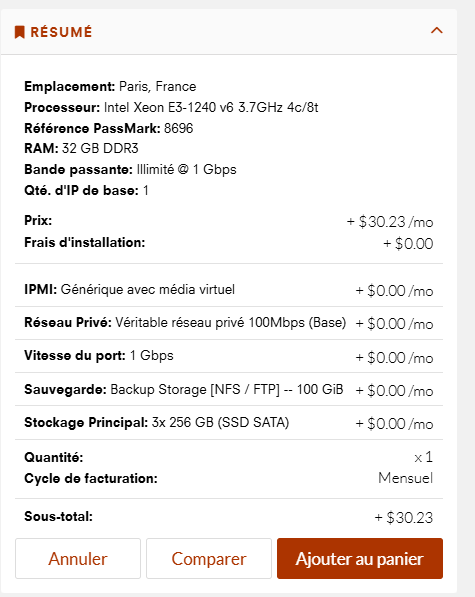
\includegraphics[width=0.5\textwidth]{figures/captures/real_serveur_offre.png}
    \caption{Configuration du serveur retenu à la commande}
    \label{fig:real_serveur}
\end{figure}

À l'installation du système, nous avons réservé le premier disque au système (\texttt{/boot}, 8~Go de \textit{swap}, racine). Les deux autres disques reçoivent les données Docker et les fichiers Excel importés (Figure~\ref{fig:real_partitionnement}). Un disque saturé par les images Docker ne bloque donc pas le système.

\begin{figure}[H]
    \centering
    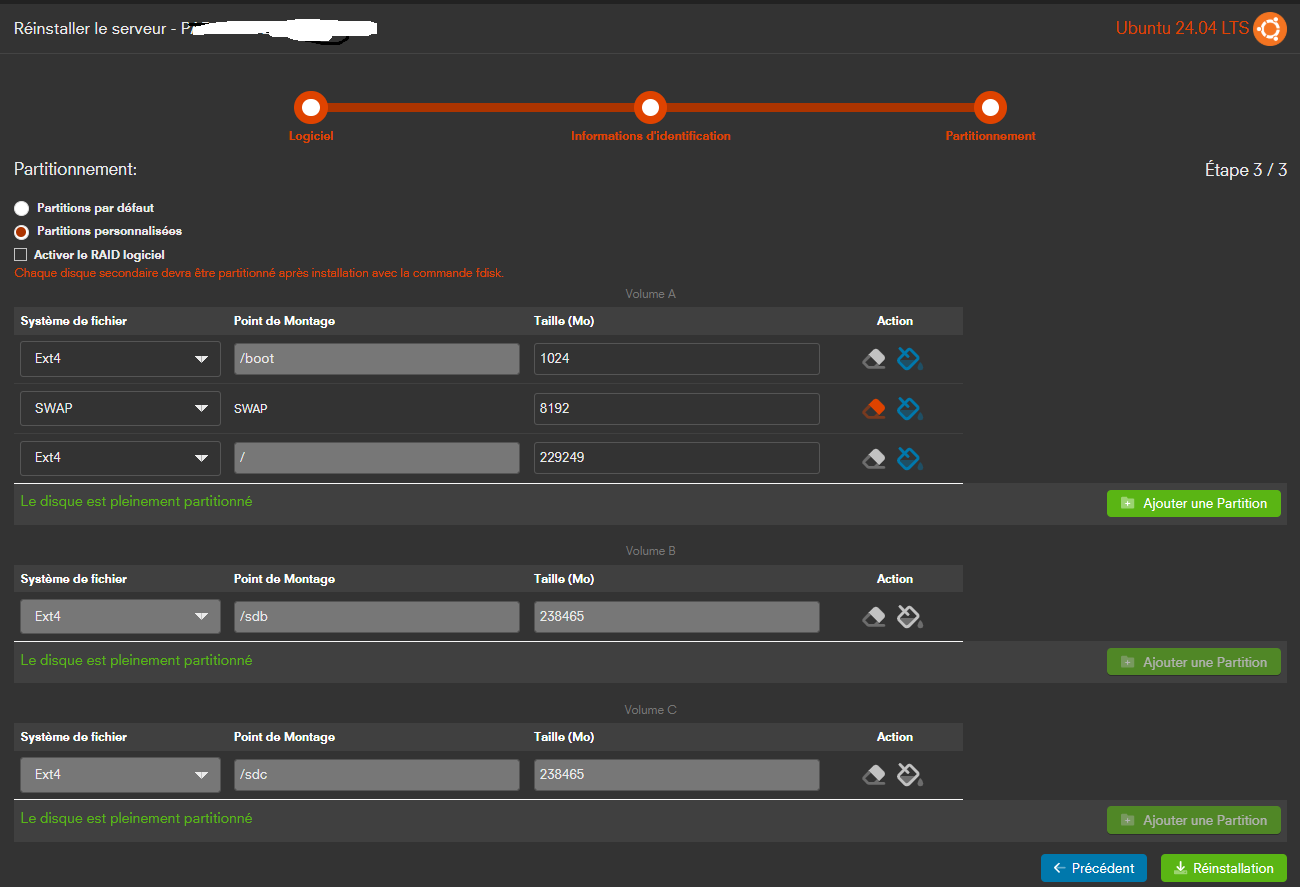
\includegraphics[width=0.85\textwidth]{figures/captures/real_partitionnement.png}
    \caption{Partitionnement des trois disques à l'installation d'Ubuntu 24.04 LTS}
    \label{fig:real_partitionnement}
\end{figure}

Le tableau~\ref{tab:env_versions} liste les composants logiciels en production et leur version, relevées directement sur le serveur. Les commandes de relevé figurent en annexe~\ref{annexe:deploiement}.

\begin{table}[H]
\centering
\footnotesize
\caption{Composants logiciels en production (relevé du 27~septembre~2026)}
\label{tab:env_versions}
\begin{tabularx}{\linewidth}{|l|X|l|}
\hline
\rowcolor[HTML]{EFEFEF}
\textbf{Composant} & \textbf{Rôle} & \textbf{Version} \\ \hline
Docker Engine / Compose & Conteneurisation et orchestration mono-hôte & 29.8.1 / 5.5.1 \\ \hline
PostgreSQL + pgvector & Base relationnelle et vectorielle & 16.15 / 0.8.6 \\ \hline
Apache Airflow & Orchestration du pipeline ETL & 2.7.3 \\ \hline
Python & Service RAG local (FastAPI) et ETL & 3.11.16 \\ \hline
Ollama / Mistral~7B & Inférence locale & 0.34.4 / 7B \\ \hline
n8n & Orchestration du routage hybride & 2.40.7 \\ \hline
Node.js & Backend Express & 20.20.2 \\ \hline
GitLab Runner & Exécution des pipelines CI/CD & 19.4.1 \\ \hline
\end{tabularx}
\end{table}

Le code est réparti en deux dépôts GitLab. Le premier, \texttt{assistant-soyaff}, porte le DAG Airflow, l'API RAG, le workflow n8n et les migrations de la base (Figure~\ref{fig:real_arbo_ia}). Le second, \texttt{assistant-soyaff-app}, porte le backend Express et le frontend React (Figure~\ref{fig:real_arbo_app}). Chaque dépôt a son propre pipeline de déploiement (\S\ref{sec:devops_cicd}).

\begin{figure}[H]
    \centering
    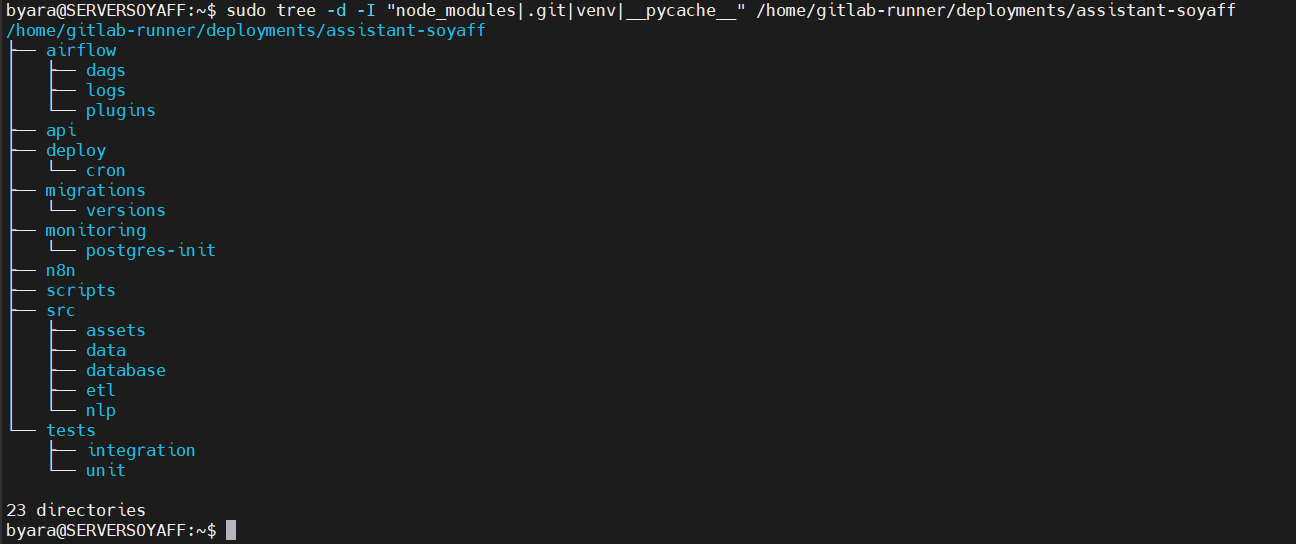
\includegraphics[width=0.75\textwidth]{figures/captures/real_arbo_ia.png}
    \caption{Arborescence du dépôt \texttt{assistant-soyaff} déployé sur le serveur}
    \label{fig:real_arbo_ia}
\end{figure}

\begin{figure}[H]
    \centering
    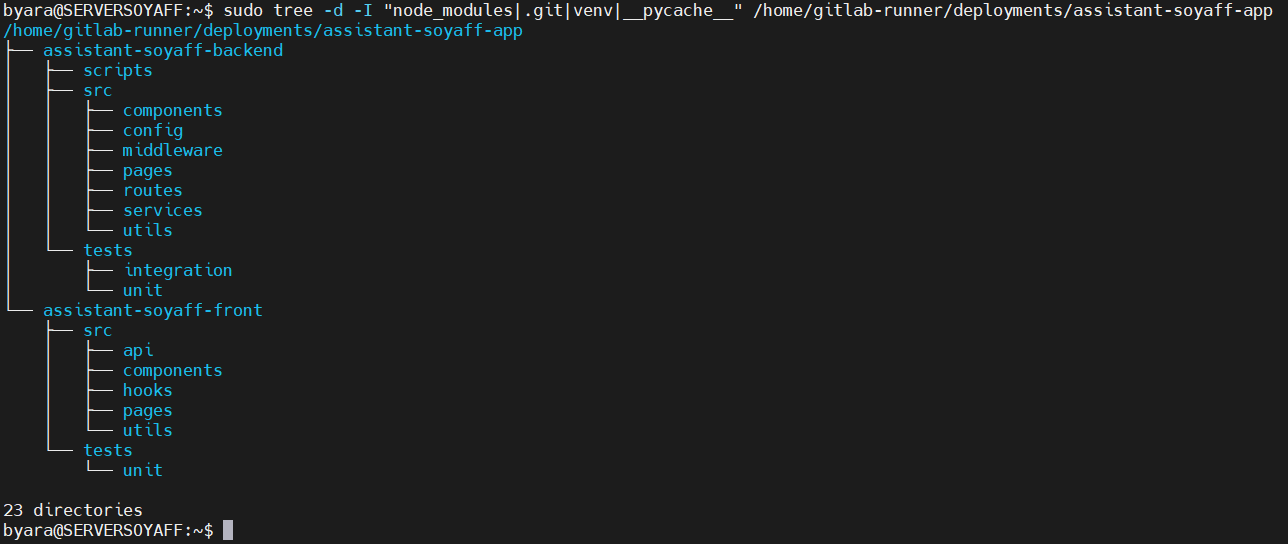
\includegraphics[width=0.75\textwidth]{figures/captures/real_arbo_app.png}
    \caption{Arborescence du dépôt \texttt{assistant-soyaff-app} déployé sur le serveur}
    \label{fig:real_arbo_app}
\end{figure}

\section{Pipeline ETL (Apache Airflow)}
\label{chap:etl}
Cette section décrit le pipeline qui alimente la plateforme à partir des fichiers tableurs historiques de SOYAFF. Il réalise les exigences \texttt{EF-ETL-01} (import de l'historique) et \texttt{EF-ETL-02} (absence de doublon), sous la contrainte de volume \texttt{ENF-VOL-01}. Le choix d'Airflow est justifié par l'ADR-01 (\S\ref{sec:adr}) ; nous nous concentrons ici sur les décisions imposées par la nature réelle des données.

\subsection{Architecture du pipeline et granularité d'orchestration}
\label{sec: architecture-pipeline}

Le DAG \texttt{etl\_excel\_to\_postgres} enchaîne deux tâches (Figure~\ref{fig:etl_dag}). La première, \texttt{run\_excel\_etl}, regroupe dans une seule fonction Python l'extraction, la transformation et le chargement. La seconde, \texttt{generate\_embeddings}, relit les transactions en base et calcule leurs vecteurs dans la table \texttt{transport\_embeddings}, hébergée dans la même instance PostgreSQL (ADR-04). Les deux tâches ne s'échangent aucune donnée en mémoire : leur seule frontière est l'état persisté en base.

\begin{figure}[H]
    \centering
    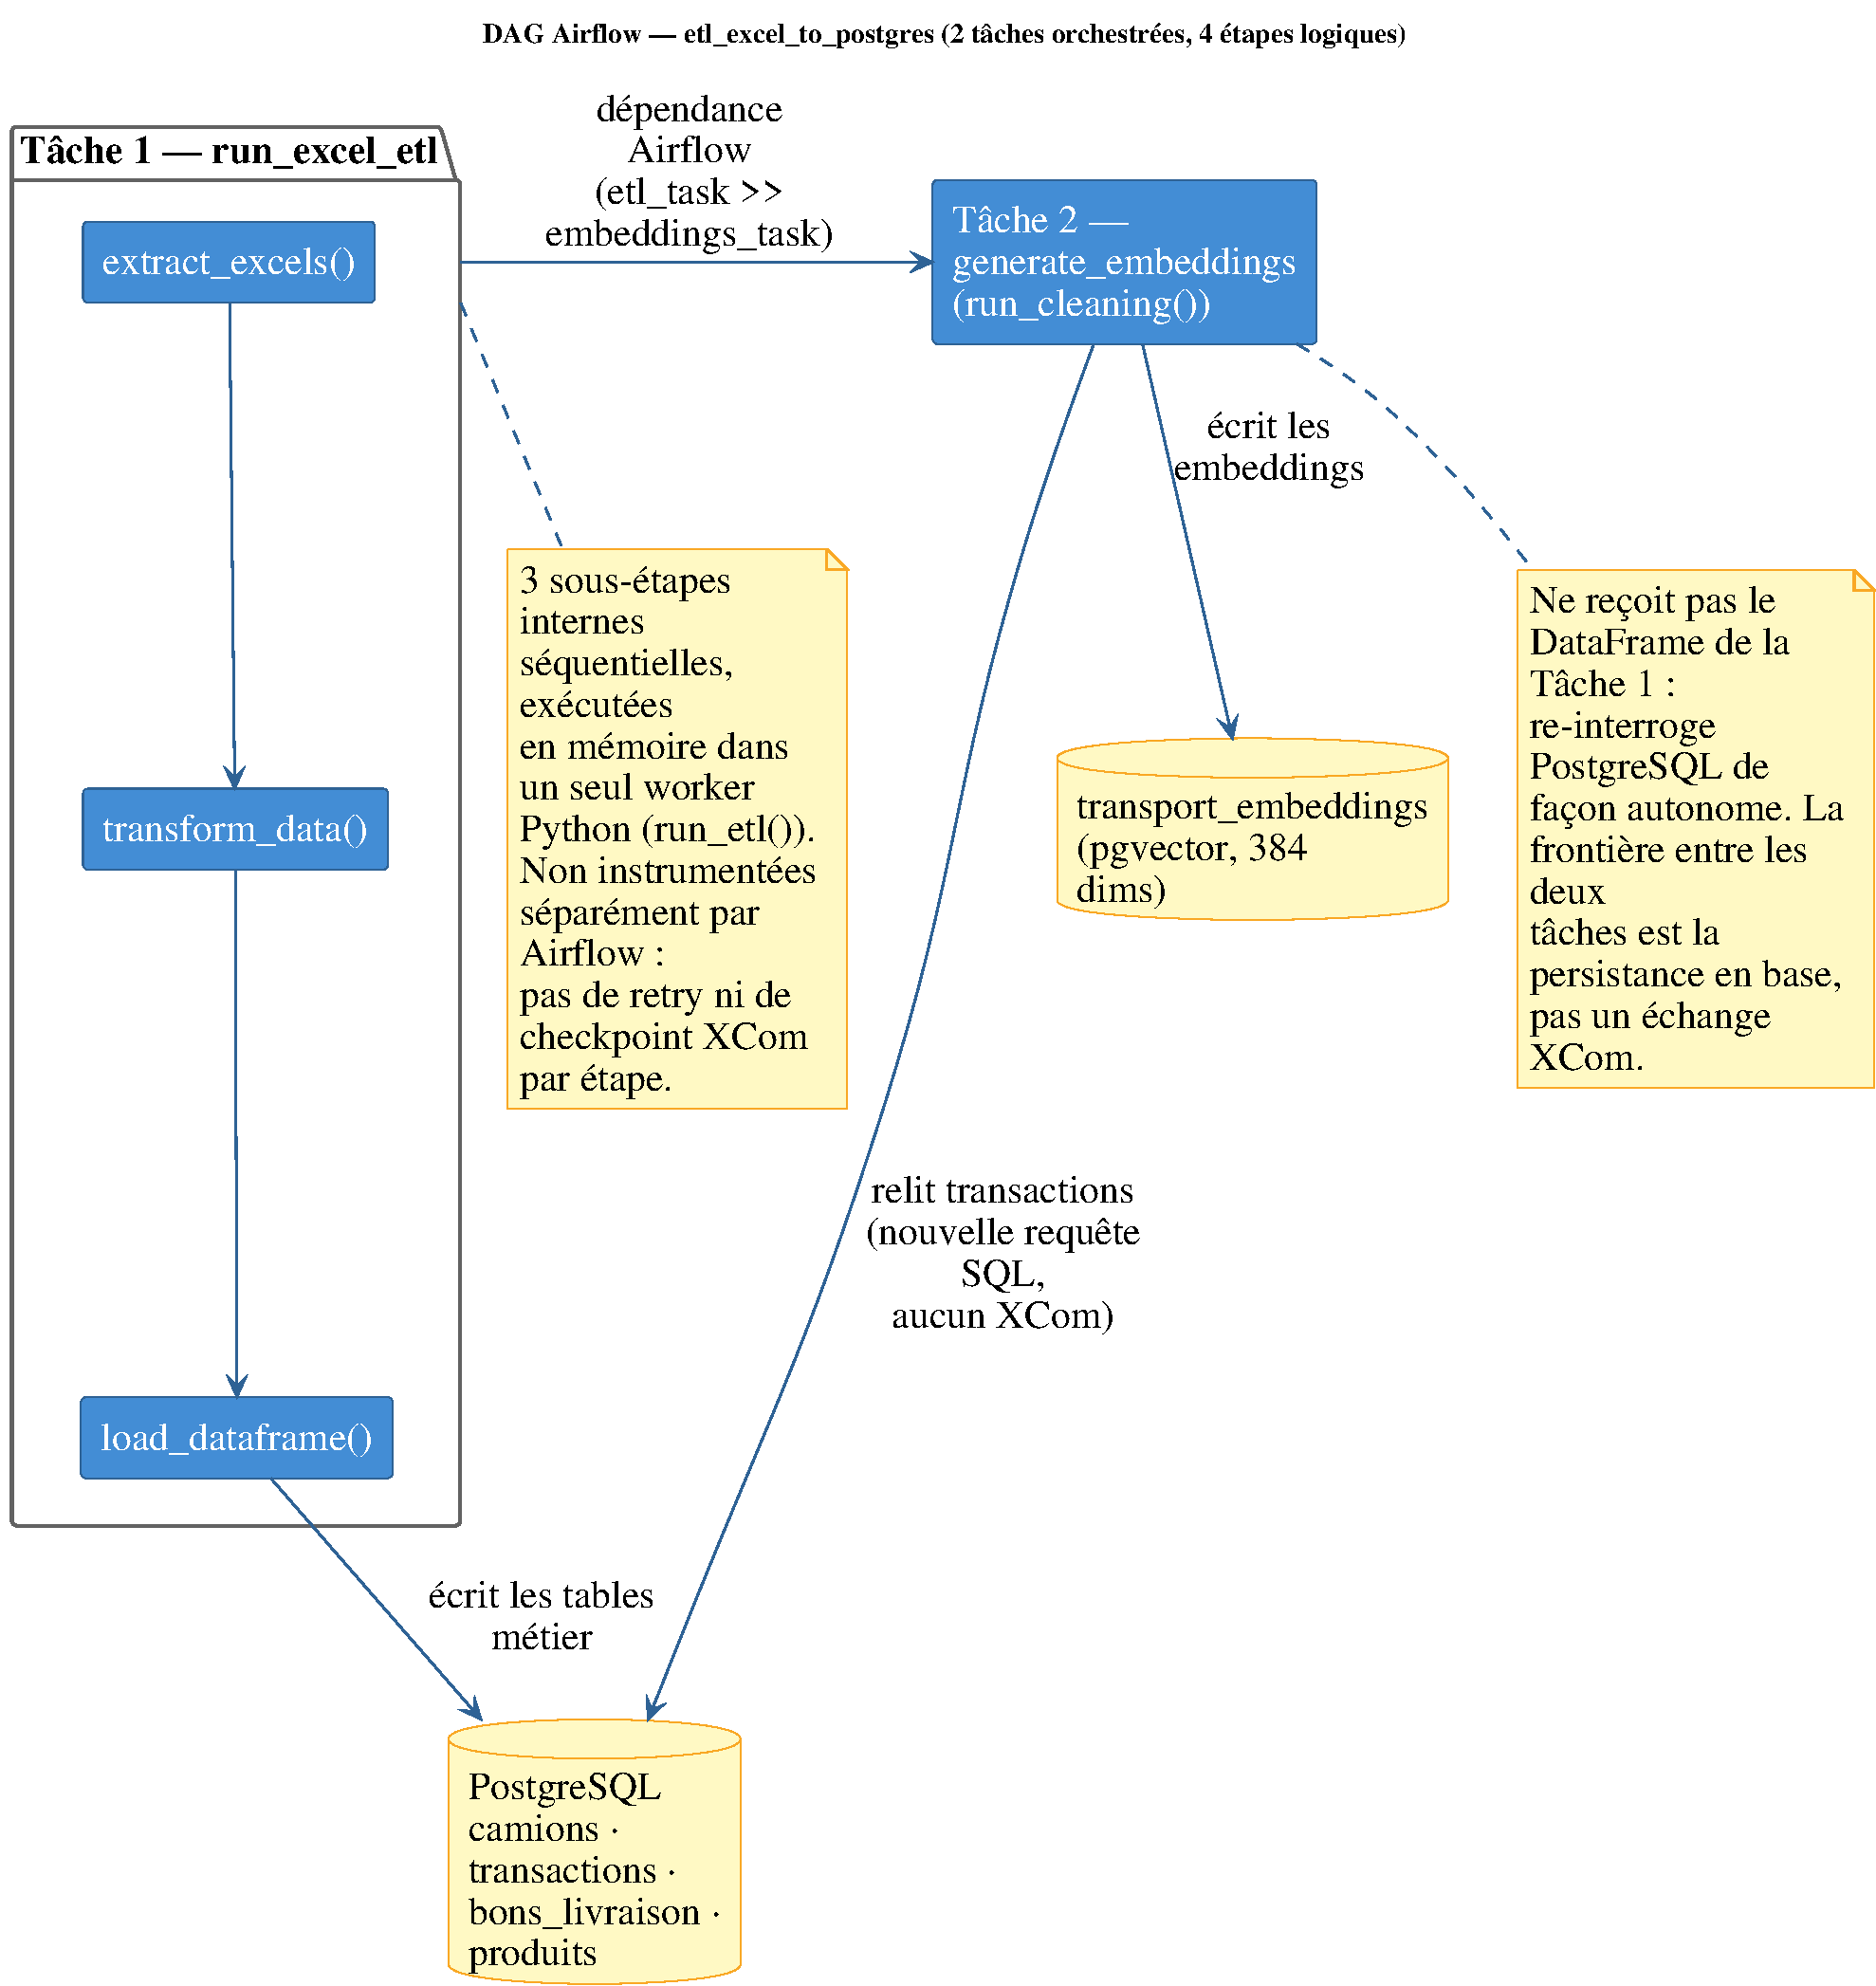
\includegraphics[width=\textwidth,height=0.88\textheight,keepaspectratio]{figures/fig_etl_dag.pdf}
    \caption{DAG Airflow \texttt{etl\_excel\_to\_postgres}, deux tâches orchestrées, quatre étapes logiques}
    \label{fig:etl_dag}
    \source{Schéma de l'auteur}
\end{figure}

\textbf{Pourquoi deux tâches, et pas quatre.} Découper extraction, transformation et chargement en trois tâches Airflow aurait obligé à faire transiter plusieurs milliers de lignes par \texttt{XCom}, un mécanisme qui n'est pas prévu pour ces volumes. Les regrouper garde les données en mémoire. Le prix est qu'un échec au chargement fait rejouer toute la tâche ; c'est sans danger, car l'extraction et la transformation sont rejouables à l'identique et le chargement est idempotent (\S\ref{sec: chargement}). La vectorisation, elle, est isolée pour une autre raison : c'est une charge de calcul, treize fois plus lente que le chargement (3~min~50 contre 17~s), qui mérite son propre suivi.

\textbf{Un déclenchement à la demande.} Les fichiers Excel contiennent des données personnelles : ils ne sont jamais versionnés, conformément à la loi n\textsuperscript{o}~2008-12 \cite{senegalLoi200812}. Un script transfère les fichiers vers le serveur par une liaison chiffrée, puis déclenche le DAG par l'API d'Airflow. Le DAG n'a donc pas de planification récurrente : il s'exécute à chaque dépôt de fichier.

\subsection{Extraction : absorber l'hétérogénéité des sources}
\label{sec: extraction}

L'informalité documentaire décrite dans l'état de l'art se lit dans chaque fichier. Les noms portent des doubles espaces ou un suffixe \texttt{- Copie} : aucune convention de nommage ne peut être présumée. Chaque feuille commence par une ligne de titre libre, suivie de deux lignes d'en-tête superposées. Les feuilles sont donc lues comme une grille brute, sans en-tête ; les noms de colonnes sont reconstitués à la transformation.

Les fichiers sont triés par ordre chronologique à partir du mois et de l'année lus dans leur nom. Un tri alphabétique placerait \textit{AOUT} avant \textit{AVRIL} et \textit{JANVIER}. Or la date d'émission d'un bon de livraison est fixée à sa première occurrence : sans ce tri, elle dépendrait de l'ordre des fichiers sur le disque, une corruption silencieuse. Chaque ligne est enfin étiquetée avec son fichier et sa feuille d'origine, pour l'audit et pour la clé de déduplication.

\subsection{Transformation et normalisation}
\label{sec: transformation}

\texttt{transform\_data()} impose un schéma unique en six étapes, chacune répondant à un défaut réel des classeurs :
\begin{enumerate}
    \item les deux lignes d'en-tête sont fusionnées en noms de colonnes (« Extrait » et « N° » deviennent \texttt{extrait\_n}) ;
    \item chaque colonne est reconnue par un motif sur son nom (\texttt{date}, \texttt{libell[eé]}, \texttt{camion}\ldots), et non par sa position, qui varie entre récapitulatifs mensuels et journaliers ; l'absence d'une colonne obligatoire arrête le traitement avec un message explicite ;
    \item les montants notés à la française (« 1.700.000 CFA ») sont convertis en nombres ;
    \item les dates sont lues au format jour/mois (\texttt{dayfirst=True}), sans quoi le 03/04 deviendrait le 4 mars ;
    \item les lignes « report solde », qui reportent un cumul d'une page à l'autre, sont écartées : elles fausseraient les totaux ;
    \item la clé de déduplication \texttt{source\_key} est calculée, après nettoyage, pour qu'un même montant écrit de deux façons produise la même clé.
\end{enumerate}

\subsection{Chargement idempotent}
\label{sec: chargement}

\textbf{La clé \texttt{source\_key}} est l'empreinte MD5 de neuf champs :
\[
\begin{aligned}
\texttt{source\_key} = \mathrm{MD5}\big(\;
  &\texttt{source\_file} \,\|\, \texttt{source\_sheet} \,\|\, \texttt{date\_transaction} \,\|\,{} \\
  &\texttt{libelle} \,\|\, \texttt{entrees\_appro} \,\|\, \texttt{sorties\_depenses} \,\|\,{} \\
  &\texttt{solde\_progressif} \,\|\, \texttt{camion\_raw} \,\|\, \texttt{bl\_raw}\;\big)
\end{aligned}
\]
Le fichier et la feuille séparent deux lignes identiques venues de mois différents ; le solde progressif, cumulatif, distingue deux lignes identiques d'un même fichier (plusieurs « CARBURANT GOLO » dans le mois). La colonne \texttt{source\_key} porte une contrainte d'unicité, et l'insertion utilise \texttt{ON CONFLICT (source\_key) DO NOTHING} : une ligne déjà présente est simplement comptée comme doublon. Rejouer le pipeline, entièrement ou en partie, n'insère donc aucun doublon ; c'est ce qui rend possible la reprise après une coupure de connexion (ADR-01).

\textbf{Des référentiels qui s'enrichissent.} Les tables \texttt{camions}, \texttt{bons\_livraison} et \texttt{produits} sont, elles, mises à jour à chaque import (\texttt{DO UPDATE}) : une transaction est un fait figé, un camion peut changer de statut. Un camion d'abord vu comme camion de la société peut être requalifié \texttt{particulier} par une « avance transport » ; l'inverse est interdit (Figure~\ref{fig:etl_table_camions}). Un libellé qui cite plusieurs camions est découpé et chaque camion est enregistré, mais seul le premier est rattaché à la transaction : c'est une limite du schéma. Une alerte signale les dépenses de carburant, de route, de ration ou d'amende sans camion identifié.

\begin{figure}[H]
    \centering
    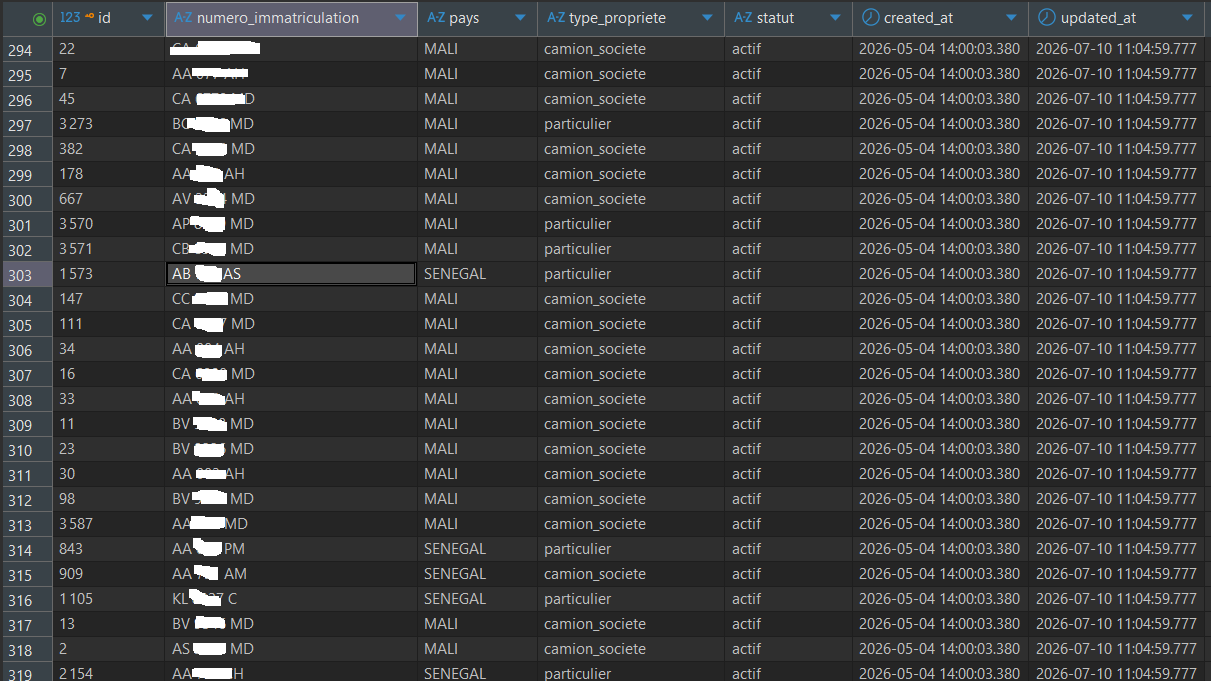
\includegraphics[width=0.8\textwidth]{figures/captures/etl_table_camions.png}
    \caption{Référentiel \texttt{camions} en base, classé par pays et type de propriété (extrait)}
    \label{fig:etl_table_camions}
\end{figure}

\begin{figure}[H]
    \centering
    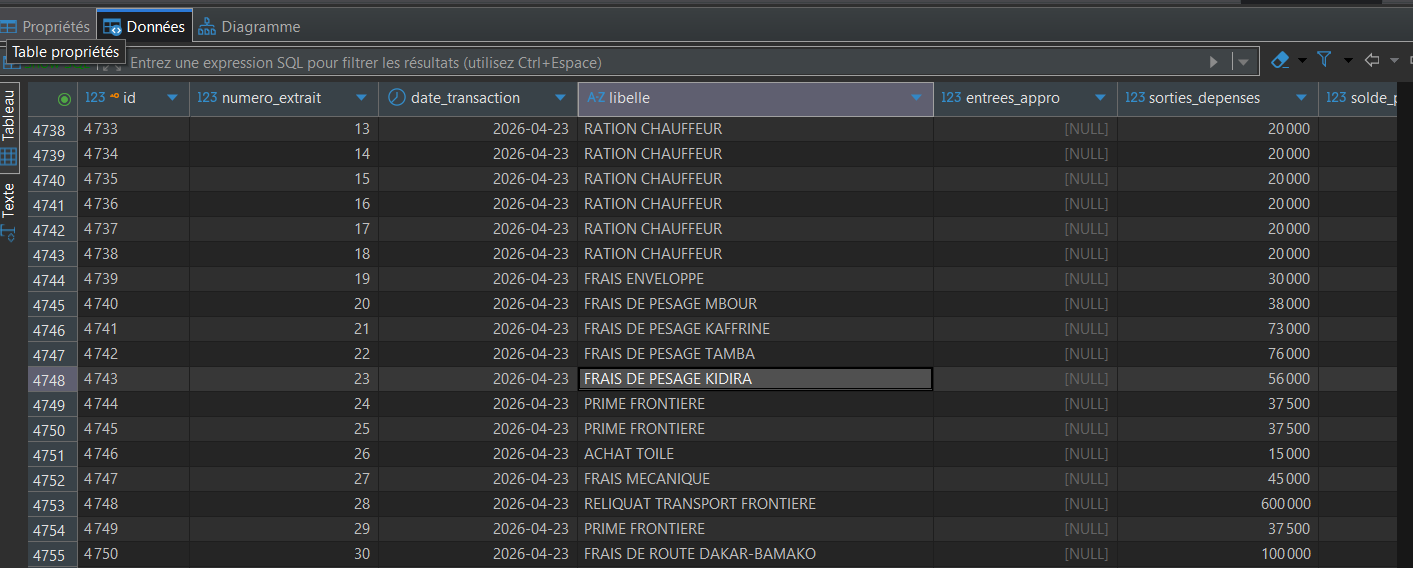
\includegraphics[width=0.8\textwidth]{figures/captures/etl_table_transactions.png}
    \caption{Transactions chargées dans PostgreSQL (extrait)}
    \label{fig:etl_table_transactions}
\end{figure}

\subsection{Vectorisation du batch ETL au corpus RAG}
\label{sec:  vectorisation}

La seconde tâche relit chaque transaction avec son camion, son bon de livraison et ses produits, compose un texte court (\textit{ex.} « Categorie carburant Camion AA~076~AH BL~1234 Produit gasoil »), puis le transforme en vecteur de 384 dimensions avec le modèle \texttt{all-MiniLM-L6-v2}. C'est le même modèle que celui qui encode les questions dans le service RAG local (\S\ref{sec:c4_composants}) : requêtes et corpus partagent le même espace. Les champs absents reçoivent une valeur explicite (\texttt{"inconnu"}) plutôt que la chaîne \texttt{"None"}. Les vecteurs sont enregistrés avec \texttt{ON CONFLICT (id) DO UPDATE} : rejouer la tâche rafraîchit les vecteurs sans les dupliquer (Figure~\ref{fig:etl_table_embeddings}).

\begin{figure}[H]
    \centering
    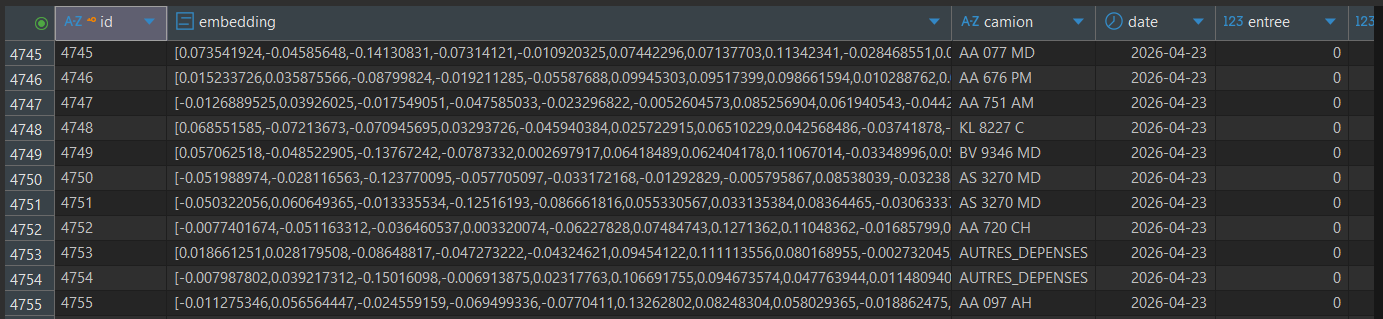
\includegraphics[width=0.8\textwidth]{figures/captures/etl_table_embeddings.png}
    \caption{Vecteurs d'embedding stockés dans \texttt{transport\_embeddings} (extrait)}
    \label{fig:etl_table_embeddings}
\end{figure}

\subsection{Validation du pipeline}
\label{sec: validation}

\textbf{Chargement initial.} Le 4~mai~2026, une exécution a ingéré 21 fichiers (15 récapitulatifs mensuels de janvier~2025 à mars~2026, 6 journaliers d'avril~2026). Elle a inséré 4~755 transactions, au-dessus du seuil de 4~500 de \texttt{ENF-VOL-01}. Les 3~595 enregistrements de camions correspondent à 319 camions distincts : un camion est compté à chaque apparition dans les transactions. Le Tableau~\ref{tab:validation_synthese} rassemble les chiffres.

\textbf{Preuve d'idempotence.} Le 10~juillet~2026, le même DAG a été relancé sur les mêmes fichiers, déjà chargés. Les deux tâches ont réussi (Figure~\ref{fig:etl_dag_rejeu}). Sur les 4~755 lignes, \textbf{4~755 ont été reconnues comme doublons et aucune n'a été insérée} (Figure~\ref{fig:etl_log_rejeu}). Les référentiels ont été mis à jour à l'identique. \texttt{EF-ETL-02} est ainsi démontrée par l'expérience, pas seulement par construction. La tâche de vectorisation compte 4~776 transactions : les 21 supplémentaires viennent de saisies de test faites dans l'application entre les deux dates (Figure~\ref{fig:etl_log_embeddings}).

\begin{figure}[H]
    \centering
    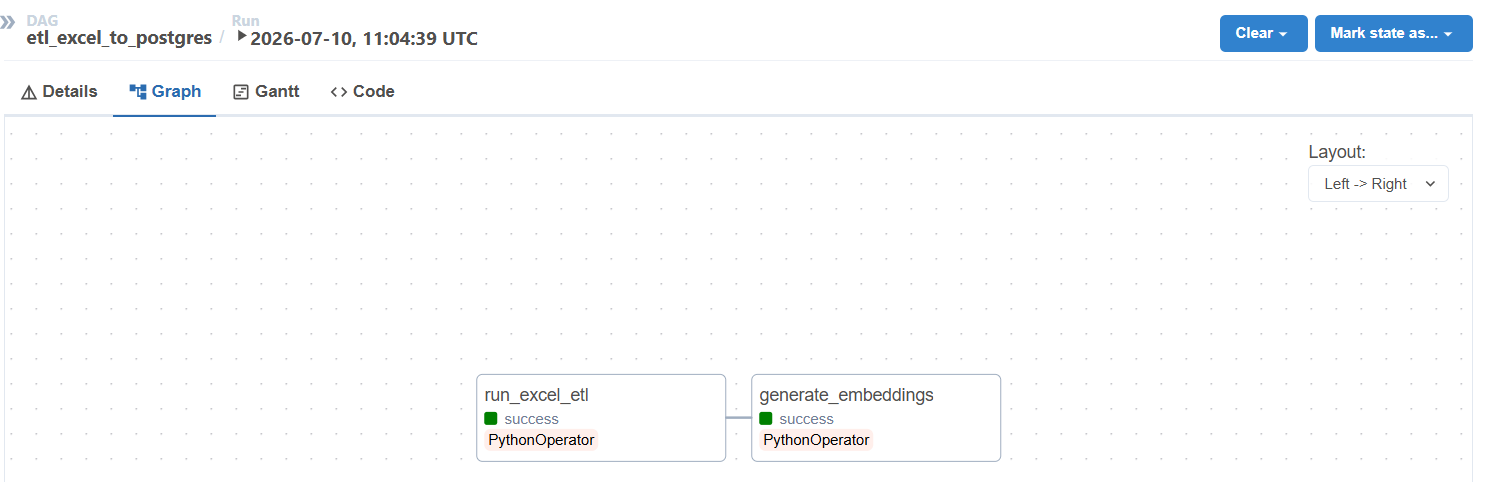
\includegraphics[width=0.8\textwidth]{figures/captures/etl_dag_rejeu.png}
    \caption{Rejeu de contrôle du 10~juillet~2026 dans Airflow : les deux tâches en succès}
    \label{fig:etl_dag_rejeu}
\end{figure}

\begin{figure}[H]
    \centering
    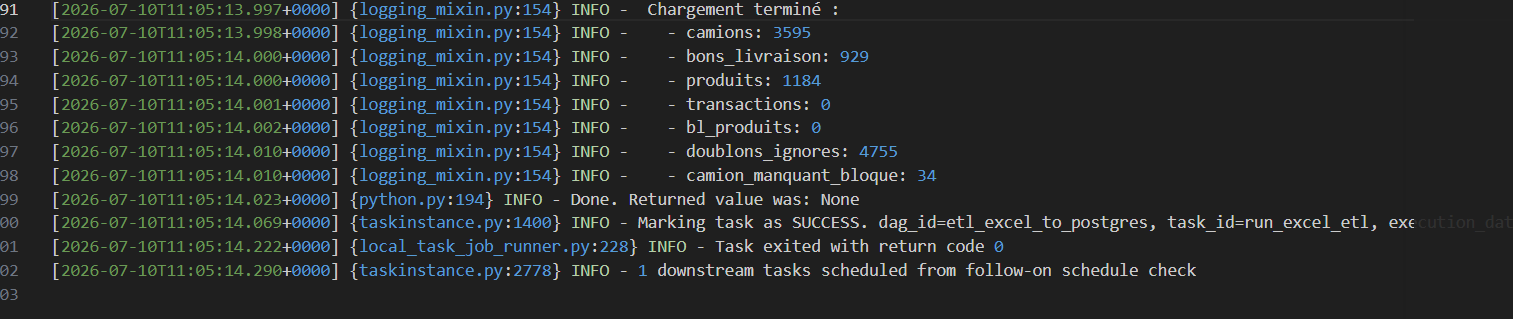
\includegraphics[width=0.95\textwidth]{figures/captures/etl_log_rejeu.png}
    \caption{Journal de la tâche \texttt{run\_excel\_etl} au rejeu : 0 transaction insérée, 4~755 doublons ignorés}
    \label{fig:etl_log_rejeu}
\end{figure}

\begin{figure}[H]
    \centering
    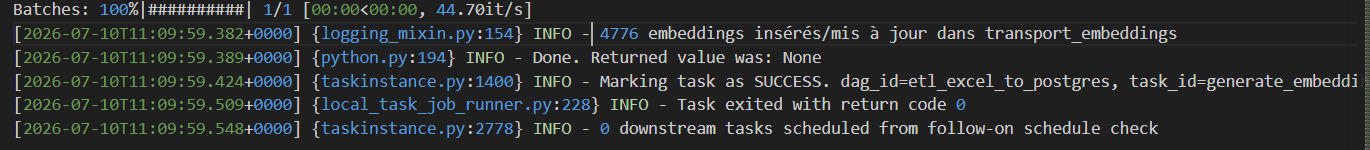
\includegraphics[width=0.95\textwidth]{figures/captures/etl_log_embeddings.png}
    \caption{Journal de la tâche \texttt{generate\_embeddings} au rejeu : 4~776 embeddings insérés ou mis à jour}
    \label{fig:etl_log_embeddings}
\end{figure}

\textbf{Rejets et durée.} L'extraction produit 5~023 lignes brutes ; 268 sont écartées (5,3~\%) : reports de solde, lignes sans date ou sans libellé, lignes de titre des fichiers suivant le premier. Le pipeline ne distingue pas ces causes : leur répartition n'est pas mesurée. Les 34 dépenses sans camion identifié sont chargées avec une alerte, pas rejetées. Le DAG complet s'exécute en moins de 4~min~35, ce qui permet un traitement après chaque dépôt de fichier.

\begin{table}[htbp]
\centering
\footnotesize
\caption{Validation du pipeline : chargement initial (04/05/2026) et rejeu de contrôle (10/07/2026)}
\label{tab:validation_synthese}
\begin{tabularx}{\linewidth}{|>{\raggedright\arraybackslash}X|>{\raggedright\arraybackslash}p{3.0cm}|>{\raggedright\arraybackslash}p{3.4cm}|}
\hline
\rowcolor[HTML]{EFEFEF}
\textbf{Métrique} & \textbf{Valeur mesurée} & \textbf{Exigence / statut} \\ \hline
Fichiers ingérés & 21 & \\ \hline
Transactions insérées & 4~755 & \texttt{ENF-VOL-01} ($\geq$~4~500) : dépassé \\ \hline
Camions : enregistrements / distincts & 3~595 / 319 & \\ \hline
Bons de livraison : enregistrements / distincts & 929 / 727 & \\ \hline
Produits : enregistrements / distincts & 1~184 / 633 & \\ \hline
Doublons reconnus au rejeu & 4~755 / 4~755 & \texttt{EF-ETL-02} : prouvé \\ \hline
Transactions insérées au rejeu & 0 & \texttt{EF-ETL-02} : prouvé \\ \hline
Lignes écartées & 268 / 5~023 (5,3~\%) & causes non ventilées \\ \hline
Dépenses sans camion identifié & 34 & chargées avec alerte \\ \hline
Durée : chargement / vectorisation / DAG & 17~s / 3~min~50 / 4~min~35 & \\ \hline
\end{tabularx}
\end{table}

\subsection{Synthèse et transition}
\label{sec: synthese-transition}

Le pipeline transforme des classeurs hétérogènes en une base relationnelle et vectorielle cohérente, qu'on peut rejouer sans risque. Il satisfait \texttt{EF-ETL-01}, \texttt{EF-ETL-02} et \texttt{ENF-VOL-01}. La section suivante décrit l'application web qui met ces données entre les mains des utilisateurs.

\section{Application web full-stack}
\label{chap:webapp}

L'application web expose aux utilisateurs de SOYAFF la base consolidée par le pipeline ETL (section~\ref{chap:etl}). Elle repose sur React~18 côté client et Express~4 côté serveur, avec une authentification par jetons signés et trois rôles. Le module conversationnel, bien que relayé par le même backend, est traité à part (section~\ref{chap:ia_rag}).

Les captures établissent que chaque fonctionnalité existe et fonctionne sur le système déployé ; leur valeur pour SOYAFF est mesurée au chapitre~\ref{chap:evaluation}. Le texte justifie les décisions qu'aucun écran ne montre. Le Tableau~\ref{tab:couverture_webapp} indique, exigence par exigence, ce qui tourne en production au 27~septembre~2026.

\begin{table}[htbp]
\centering
\footnotesize
\caption{Couverture des exigences applicatives par la réalisation (état au 27~septembre~2026)}
\label{tab:couverture_webapp}
\begin{tabularx}{\linewidth}{|>{\raggedright\arraybackslash}p{2.0cm}|>{\raggedright\arraybackslash}p{3.1cm}|>{\raggedright\arraybackslash}X|>{\raggedright\arraybackslash}p{1.5cm}|}
\hline
\rowcolor[HTML]{EFEFEF}
\textbf{Exigence} & \textbf{Fonctionnalité} & \textbf{Réalisation} & \textbf{État} \\ \hline

\texttt{EF-DSH-01} & Suivi de caisse en temps réel & \texttt{GET /api/stats} (lecture seule, agrégats parallèles) & \textbf{Déployé} \\ \hline
\texttt{EF-DSH-02}, \texttt{EF-DSH-04} & Visualisation de la flotte, profil véhicule & \texttt{CamionsPage.jsx} : liste, filtres, détail via \texttt{GET /api/camions} et \texttt{GET /api/camions/:id} & \textbf{Déployé} \\ \hline
\texttt{EF-DSH-03} & Classification société / particulier & Affichage typé (\texttt{type\_propriete}), bascule société~$\rightarrow$~particulier gérée à l'upsert & \textbf{Déployé} \\ \hline
\texttt{EF-SDR-01} & Saisie directe d'une opération financière & Page \texttt{SaisiePage.jsx} (\texttt{OperationForm.jsx}) $\rightarrow$ \texttt{POST /api/finances/operation} (transaction SQL atomique) & \textbf{Déployé} \\ \hline
\texttt{EF-SDR-02} & Contrôle des délais entre opérations d'un même camion & \texttt{utils/delais.js}, appliqué par l'API : frais de route bloqués sous 8~jours ; rations bloquées sous 2~jours, alerte à confirmer entre 2 et 5~jours ; forçage réservé à l'administrateur, tracé & \textbf{Déployé} \\ \hline
\texttt{EF-REP-01}, \texttt{EF-REP-02} & Récapitulatif journalier et mensuel consolidé & \texttt{GET /api/rapports/mois}, \texttt{GET /api/rapports/mensuel} & \textbf{Déployé} \\ \hline
\texttt{EF-REP-03} & Export CSV / Excel / PDF & CSV conforme Excel-FR (BOM~UTF-8, séparateur~\texttt{;}) et XLSX (\texttt{exceljs}) déployés ; PDF absent côté serveur, le bouton correspondant déclenche un \texttt{window.print()} navigateur & \textbf{Partiel} \\ \hline
\texttt{EF-REP-04} & Recherche multi-critères & Filtres période / camion / catégorie (\texttt{FinancesPage.jsx}, \texttt{RapportsPage.jsx}) & \textbf{Déployé} \\ \hline
\texttt{EF-VAL-02} & Workflow de validation numérique dématérialisé & Aucun statut de workflow en base ; insertion directe et définitive de la transaction & \textbf{Cible} \\ \hline
\texttt{EF-ADM-01} & Gestion des utilisateurs et des rôles & CRUD complet (\texttt{routes/admin.js}) : création, activation/désactivation, changement de rôle & \textbf{Déployé} \\ \hline
\texttt{EF-ADM-02} & Consultation des journaux d'audit & Onglet audit \texttt{AdminPage.jsx} $\rightarrow$ \texttt{GET /api/admin/audit}, table \texttt{audit\_logs} & \textbf{Déployé} \\ \hline
\texttt{ENF-SEC-01} & Authentification par jetons signés & JWT d'accès (8~h) + jeton de rafraîchissement (7~jours, haché SHA-256 en base) & \textbf{Déployé} \\ \hline
\texttt{ENF-SEC-02} & Hachage des mots de passe & \texttt{bcrypt}, coût~12 & \textbf{Déployé} \\ \hline
\texttt{ENF-SEC-03} & Contrôle d'accès basé sur les rôles & Contrainte \texttt{CHECK} SQL + middleware \texttt{authorize()} : \texttt{DAKAR\_AGENT}, \texttt{BAMAKO\_CHEF}, \texttt{ADMIN} & \textbf{Déployé} \\ \hline
\texttt{ENF-SEC-04} & Piste d'audit des actions sensibles & Table \texttt{audit\_logs} horodatée (connexions, refus d'accès, actions admin) & \textbf{Déployé} \\ \hline
\texttt{ENF-DISP-01} & Mode dégradé hors-ligne, cache local des saisies & Aucune trace de code (pas de \textit{service worker}, pas de file d'attente locale) & \textbf{Cible} \\ \hline
\end{tabularx}
\end{table}

Le socle de sécurité et le cœur métier (saisie, tableau de bord, reporting, administration) sont déployés et utilisés en production. Un point est partiel : l'export PDF, qui n'est qu'une impression du navigateur. Deux exigences \textit{Should} restent des cibles : le workflow de validation (\texttt{EF-VAL-02}) et le mode hors-ligne (\texttt{ENF-DISP-01}). La discussion de ces écarts est renvoyée à la section~\ref{chap:discussion}.

\subsection{Architecture applicative générale}
\label{sec:webapp_architecture}

La vue de conteneurs (Figure~\ref{fig:c4_conteneurs}) situe la pile : une \textit{single-page application} React~18 consomme une API REST Express~4 adossée à PostgreSQL. Deux choix d'organisation interne, invisibles sur les diagrammes, méritent d'être justifiés.

\textbf{Côté client, pas de routeur.} La vue affichée est portée par un simple état local dans \texttt{App.jsx}. Pour sept vues fixes, un routeur n'apportait rien. Le coût est double : aucune vue n'a d'URL propre, et la garde d'accès à l'administration est répétée au point de rendu au lieu d'être centralisée. Ce second point n'ouvre pas de faille : l'API vérifie elle-même le rôle (\S\ref{sec:webapp_rbac}), et contourner l'interface ne donnerait accès qu'à un écran vide.

\textbf{Côté serveur, le SQL dans les routes.} Les gestionnaires Express exécutent leurs requêtes directement, sans couche de service. Seule l'authentification, partagée par plusieurs routes, est isolée dans \texttt{authService.js}. Introduire une couche d'abstraction pour des routes qui n'ont qu'un appelant aurait été de la sur-ingénierie ; le découpage en couches est planifié dans le suivi du projet.

\subsection{Parcours de l'utilisateur}
\label{sec:webapp_parcours}

L'utilisateur se connecte par courriel et mot de passe (Figure~\ref{fig:web_connexion}). Le menu qu'il obtient dépend de son rôle : l'onglet \textit{Administration} n'apparaît que pour le rôle \texttt{ADMIN}. Le tableau de bord (Figure~\ref{fig:ui_dashboard}) réalise \texttt{EF-DSH-01} : solde de caisse, entrées, dépenses, flotte active, classement des camions et répartition des coûts, tous calculés côté serveur. Le bouton \textit{Assistant IA} ouvre le module décrit à la section~\ref{chap:ia_rag}.

\begin{figure}[H]
    \centering
    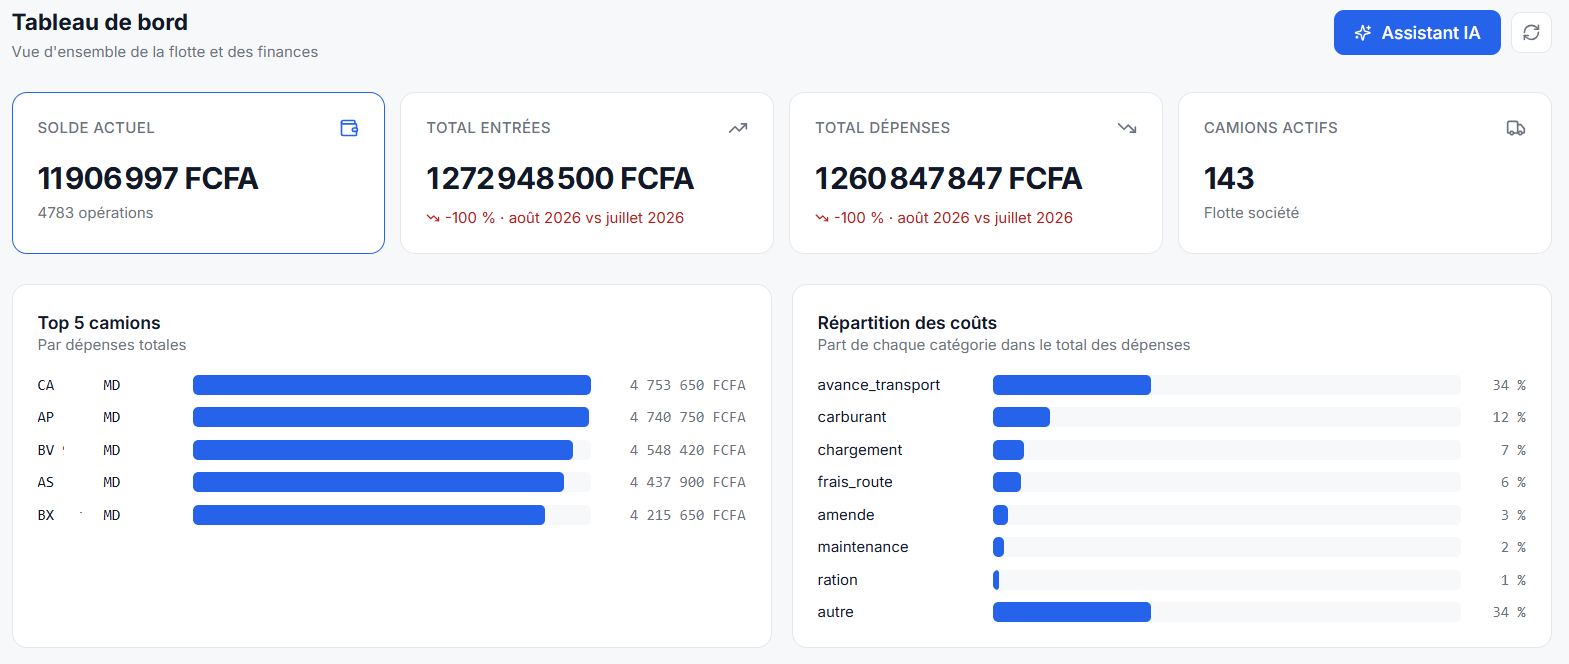
\includegraphics[width=0.85\textwidth]{figures/captures/web_dashboard.png}
    \caption{Tableau de bord : solde, entrées, dépenses, flotte active et répartition des coûts}
    \label{fig:ui_dashboard}
\end{figure}

La vue \textit{Camions} (Figure~\ref{fig:web_flotte}) réalise \texttt{EF-DSH-02} et \texttt{EF-DSH-04} : chaque carte donne l'immatriculation, le pays, la position, le total des dépenses et le nombre d'opérations, et ouvre le profil du camion.

\begin{figure}[H]
    \centering
    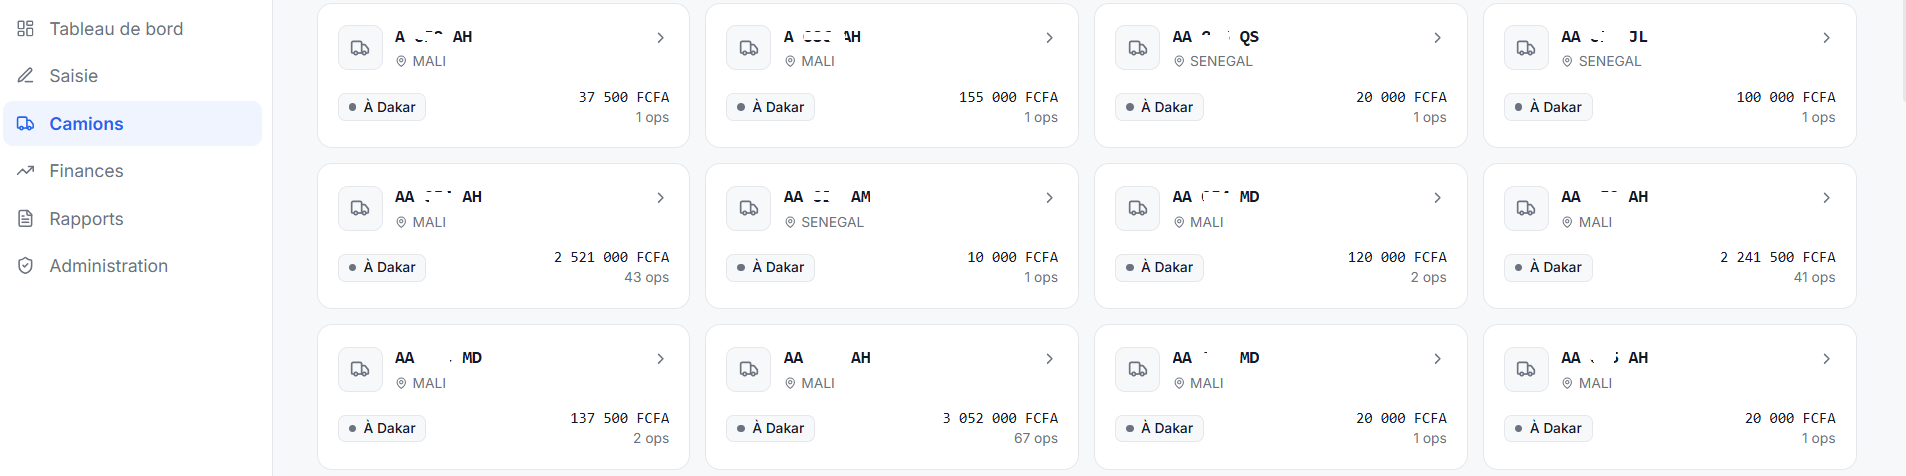
\includegraphics[width=0.85\textwidth]{figures/captures/web_flotte.png}
    \caption{Vue de la flotte par camion}
    \label{fig:web_flotte}
\end{figure}

La saisie directe (Figure~\ref{fig:web_saisie}) remplace le fichier \og RECAP-JOURNALIER \fg{} envoyé par WhatsApp. L'agent choisit le sens de l'opération, puis renseigne le libellé, la date, la catégorie, le montant et, si besoin, le camion et le bon de livraison. L'opération est visible à Bamako dès son enregistrement.

\begin{figure}[H]
    \centering
    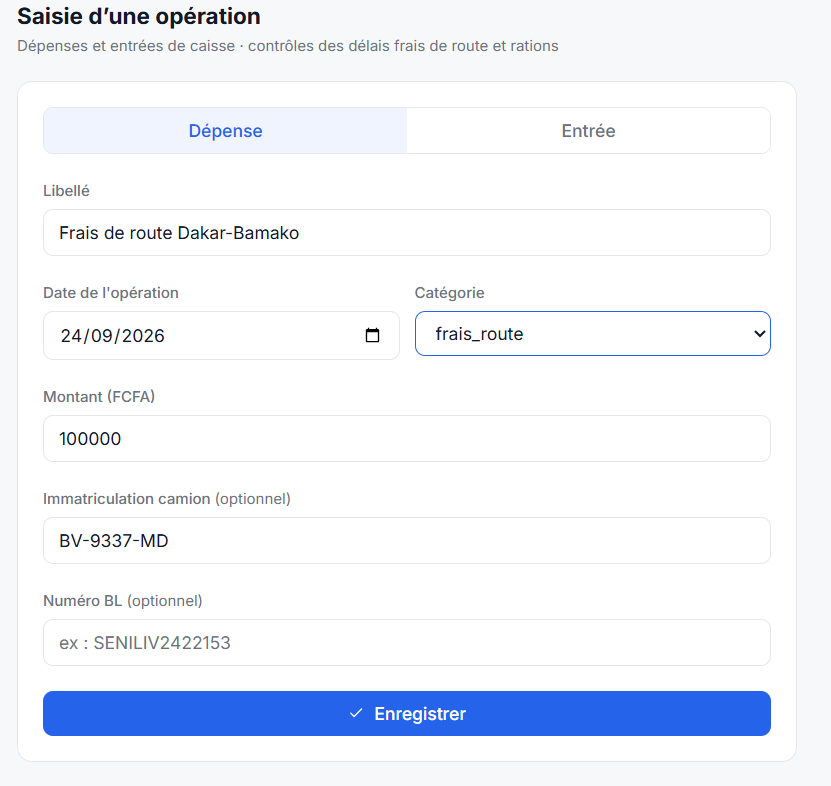
\includegraphics[width=0.5\textwidth]{figures/captures/web_saisie.png}
    \caption{Formulaire de saisie d'une opération de caisse}
    \label{fig:web_saisie}
\end{figure}

\subsection{Authentification et gestion de session}
\label{sec:webapp_jwt}

L'authentification (\texttt{ENF-SEC-01}) repose sur deux jetons. Le jeton d'accès est un JWT signé, valable huit heures ; le serveur refuse de démarrer si sa clé de signature fait moins de 64 caractères. Le jeton de rafraîchissement, valable sept jours, est une chaîne aléatoire dont seule l'empreinte SHA-256 est conservée en base : une fuite de la base ne permet donc de rejouer aucune session. Les mots de passe sont hachés par \texttt{bcrypt} (\texttt{ENF-SEC-02}).

Deux protections dépassent le cahier des charges. Un compte est verrouillé quinze minutes après cinq échecs consécutifs (Figure~\ref{fig:ui_verrouillage}). Et une adresse inconnue déclenche quand même une comparaison \texttt{bcrypt} factice : le temps de réponse ne révèle pas si un compte existe.

\begin{figure}[H]
    \centering
    \begin{minipage}{0.42\textwidth}
        \centering
        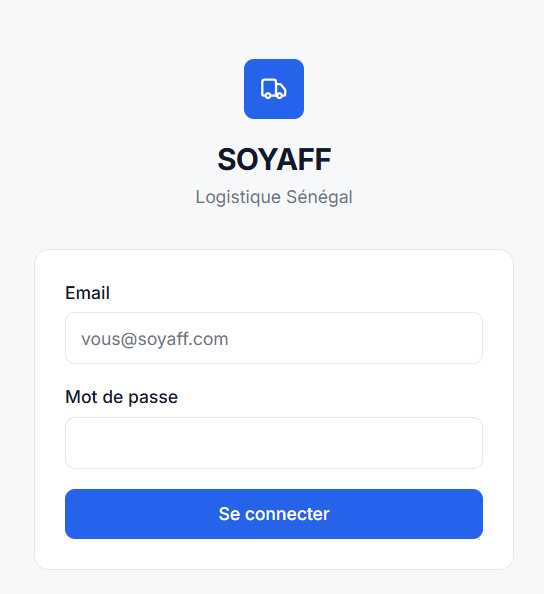
\includegraphics[width=\textwidth]{figures/captures/web_connexion.png}
        \caption{Page de connexion}
        \label{fig:web_connexion}
    \end{minipage}\hfill
    \begin{minipage}{0.48\textwidth}
        \centering
        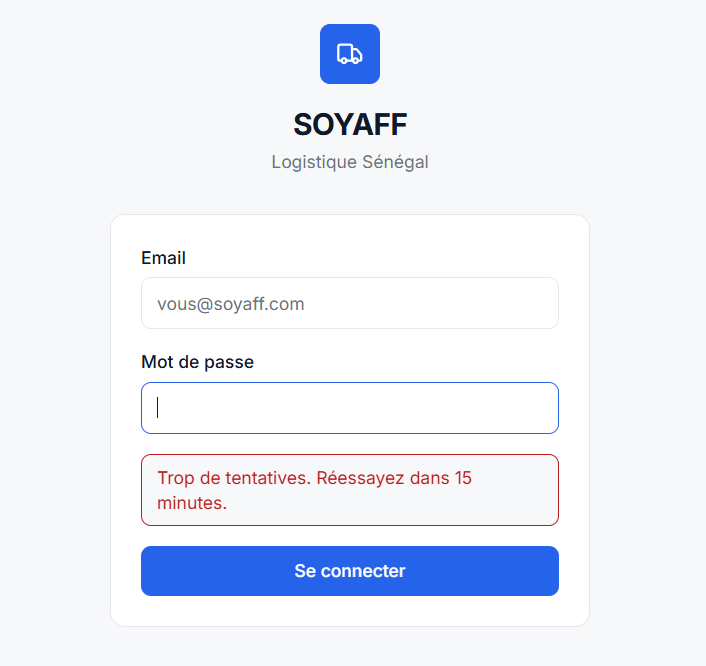
\includegraphics[width=\textwidth]{figures/captures/web_verrouillage.png}
        \caption{Compte verrouillé après cinq échecs}
        \label{fig:ui_verrouillage}
    \end{minipage}
\end{figure}

Deux arbitrages sont assumés. Les jetons sont stockés en \texttt{localStorage}, exposés à un script injecté ; la migration vers des cookies \texttt{httpOnly} est planifiée. Le jeton de rafraîchissement n'est pas renouvelé à chaque usage : il reste valable sept jours, mais la déconnexion le révoque immédiatement.

\subsection{Intégrité des données : le calcul du solde}
\label{sec:webapp_integrity}

Le diagnostic du chapitre~\ref{chap:contexte} relevait des formules de solde qui se cassaient dans les tableurs au fil des copier-coller. Le solde progressif n'est désormais calculé qu'à un seul endroit : la route de saisie \texttt{POST /api/finances/operation}, dans une transaction SQL unique. Elle garantit l'existence du camion et du bon de livraison, relit le dernier solde connu à la date de l'opération, calcule le nouveau solde et l'enregistre avec l'opération. Toute erreur annule l'ensemble : aucune opération ne peut exister sans son solde. Le frontend affiche ce solde sans jamais le recalculer. C'est le même principe que l'idempotence de l'ETL (\S\ref{sec: chargement}) : contraindre la base plutôt que discipliner l'utilisateur.

\subsection{Contrôle des délais de saisie}
\label{sec:webapp_delais}

\texttt{EF-SDR-02} demandait de contrôler l'intervalle entre deux rations d'un même chauffeur. Nous avons étendu ce contrôle aux frais de route, à la suite d'un ordre de travail du 24~septembre~2026. Les règles sont regroupées dans \texttt{utils/delais.js}, couvert par des tests :
\begin{itemize}
    \item \textbf{frais de route} : deux opérations pour un même camion doivent être espacées d'au moins 8~jours, sinon la saisie est bloquée ;
    \item \textbf{rations} : sous 2~jours, la saisie est bloquée ; entre 2 et 5~jours, l'opérateur doit confirmer une alerte.
\end{itemize}
Le chauffeur est rattaché à son camion dans la table \texttt{chauffeurs}. L'écart est mesuré par rapport à l'opération la plus proche, avant \emph{ou} après : une saisie antidatée est contrôlée comme les autres. Le contrôle s'exécute dans l'API, pas seulement dans le formulaire. Seul un administrateur peut lever un blocage ; forçage et confirmation sont inscrits dans \texttt{audit\_logs}. Les Figures~\ref{fig:web_delai_agent} et~\ref{fig:web_delai_admin} montrent la même saisie vue par un agent puis par un administrateur.

\begin{figure}[H]
    \centering
    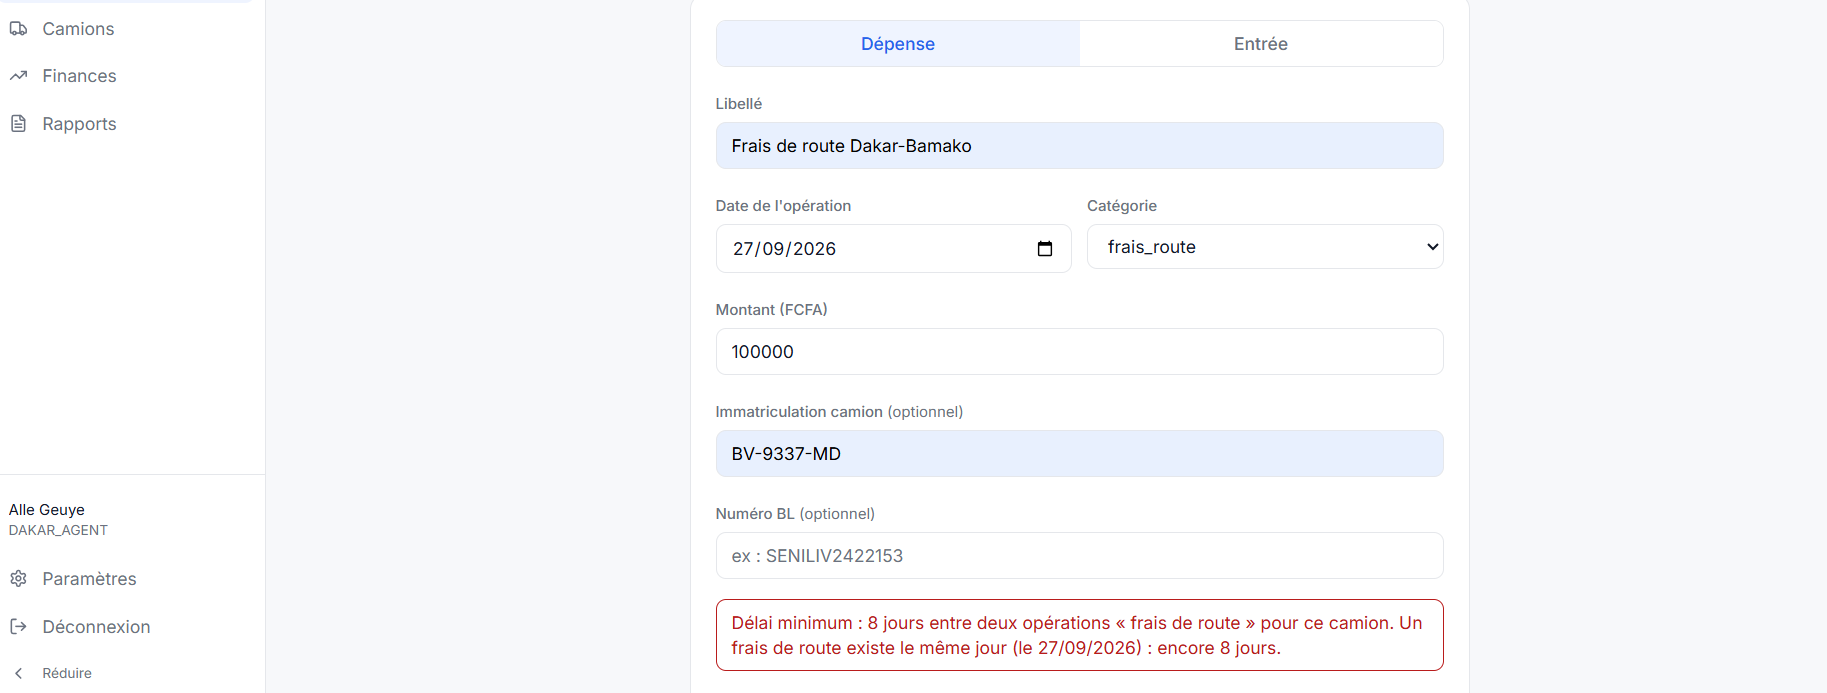
\includegraphics[width=0.8\textwidth]{figures/captures/web_delai_agent.png}
    \caption{Frais de route saisi deux fois le même jour, profil agent de Dakar : saisie bloquée}
    \label{fig:web_delai_agent}
\end{figure}

\begin{figure}[H]
    \centering
    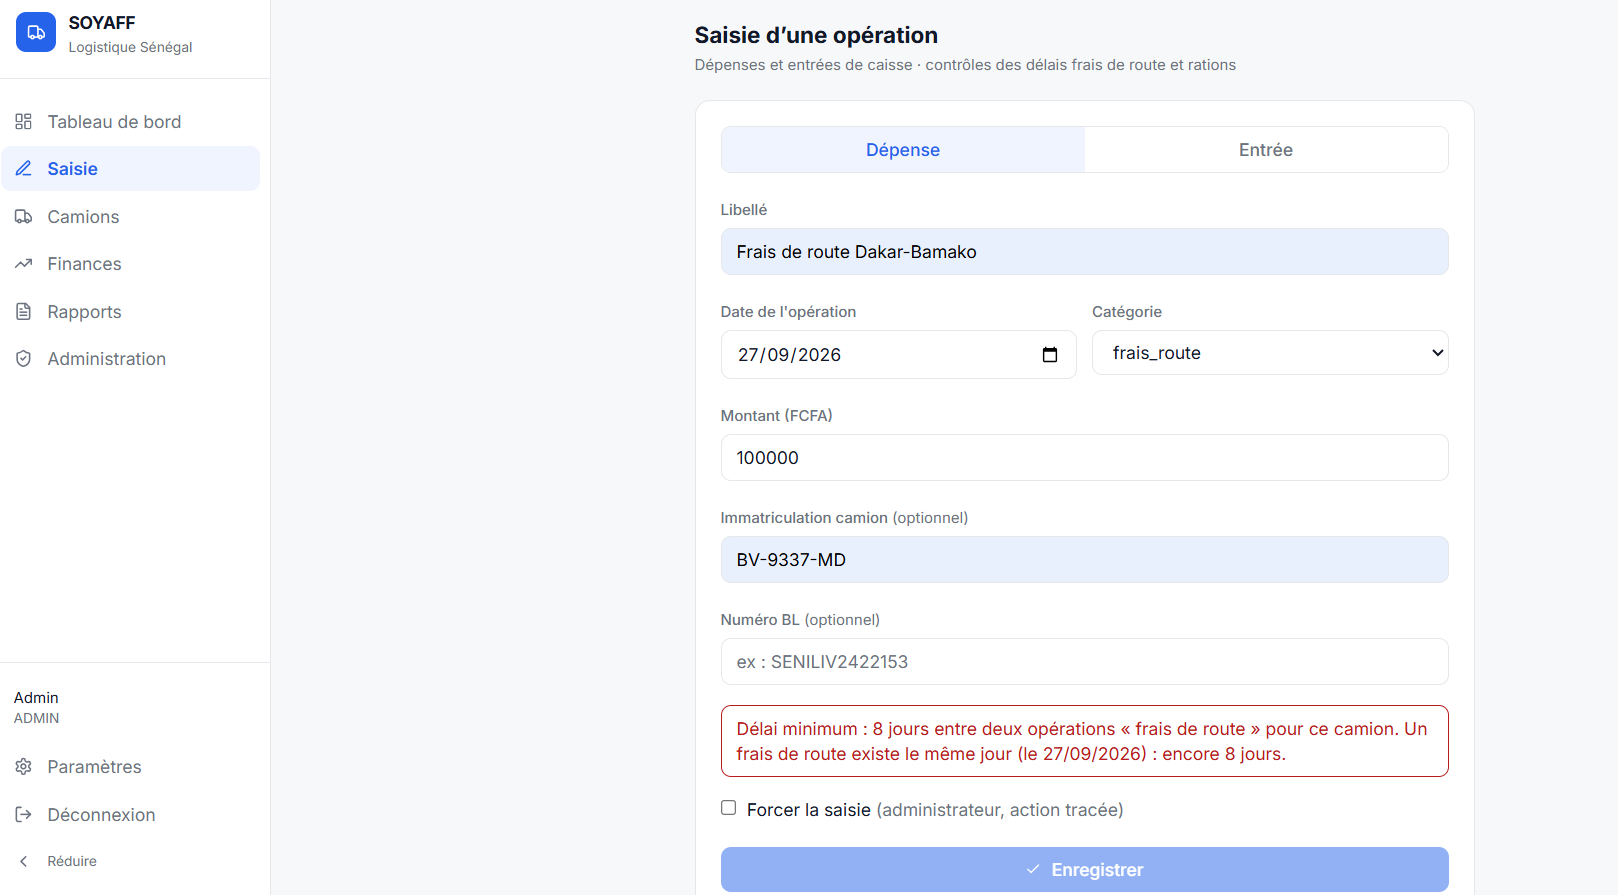
\includegraphics[width=0.7\textwidth]{figures/captures/web_delai_admin.png}
    \caption{Même saisie, profil administrateur : forçage possible et tracé}
    \label{fig:web_delai_admin}
\end{figure}

\subsection{Contrôle d'accès (RBAC) et audit}
\label{sec:webapp_rbac}

Trois rôles (\texttt{DAKAR\_AGENT}, \texttt{BAMAKO\_CHEF}, \texttt{ADMIN}) reprennent les personas de la section~\ref{chap:besoins} (\S\ref{sec:personas}). La liste est contrainte à trois niveaux : l'interface ne propose que ces valeurs, l'API rejette toute autre valeur, et une contrainte \texttt{CHECK} sur la colonne \texttt{users.role} protège la base contre toute écriture qui contournerait l'API (\texttt{ENF-SEC-03}).

Le middleware \texttt{authorize()} vérifie le rôle sur chaque route protégée. En cas de refus, il inscrit lui-même la tentative dans \texttt{audit\_logs} (\texttt{UNAUTHORIZED\_ACCESS}) avant de répondre \texttt{403}. La même table reçoit les actions d'administration réussies : création de compte, changement de rôle, réinitialisation de mot de passe (\texttt{EF-ADM-02}). Elle couvre ainsi les deux volets de \texttt{ENF-SEC-04}, résumés par la Figure~\ref{fig:seq_rbac_audit}. Un administrateur ne peut pas désactiver son propre compte ; désactiver un compte révoque ses sessions ; aucun compte n'est supprimé, pour préserver l'historique d'audit.

\begin{figure}[H]
    \centering
    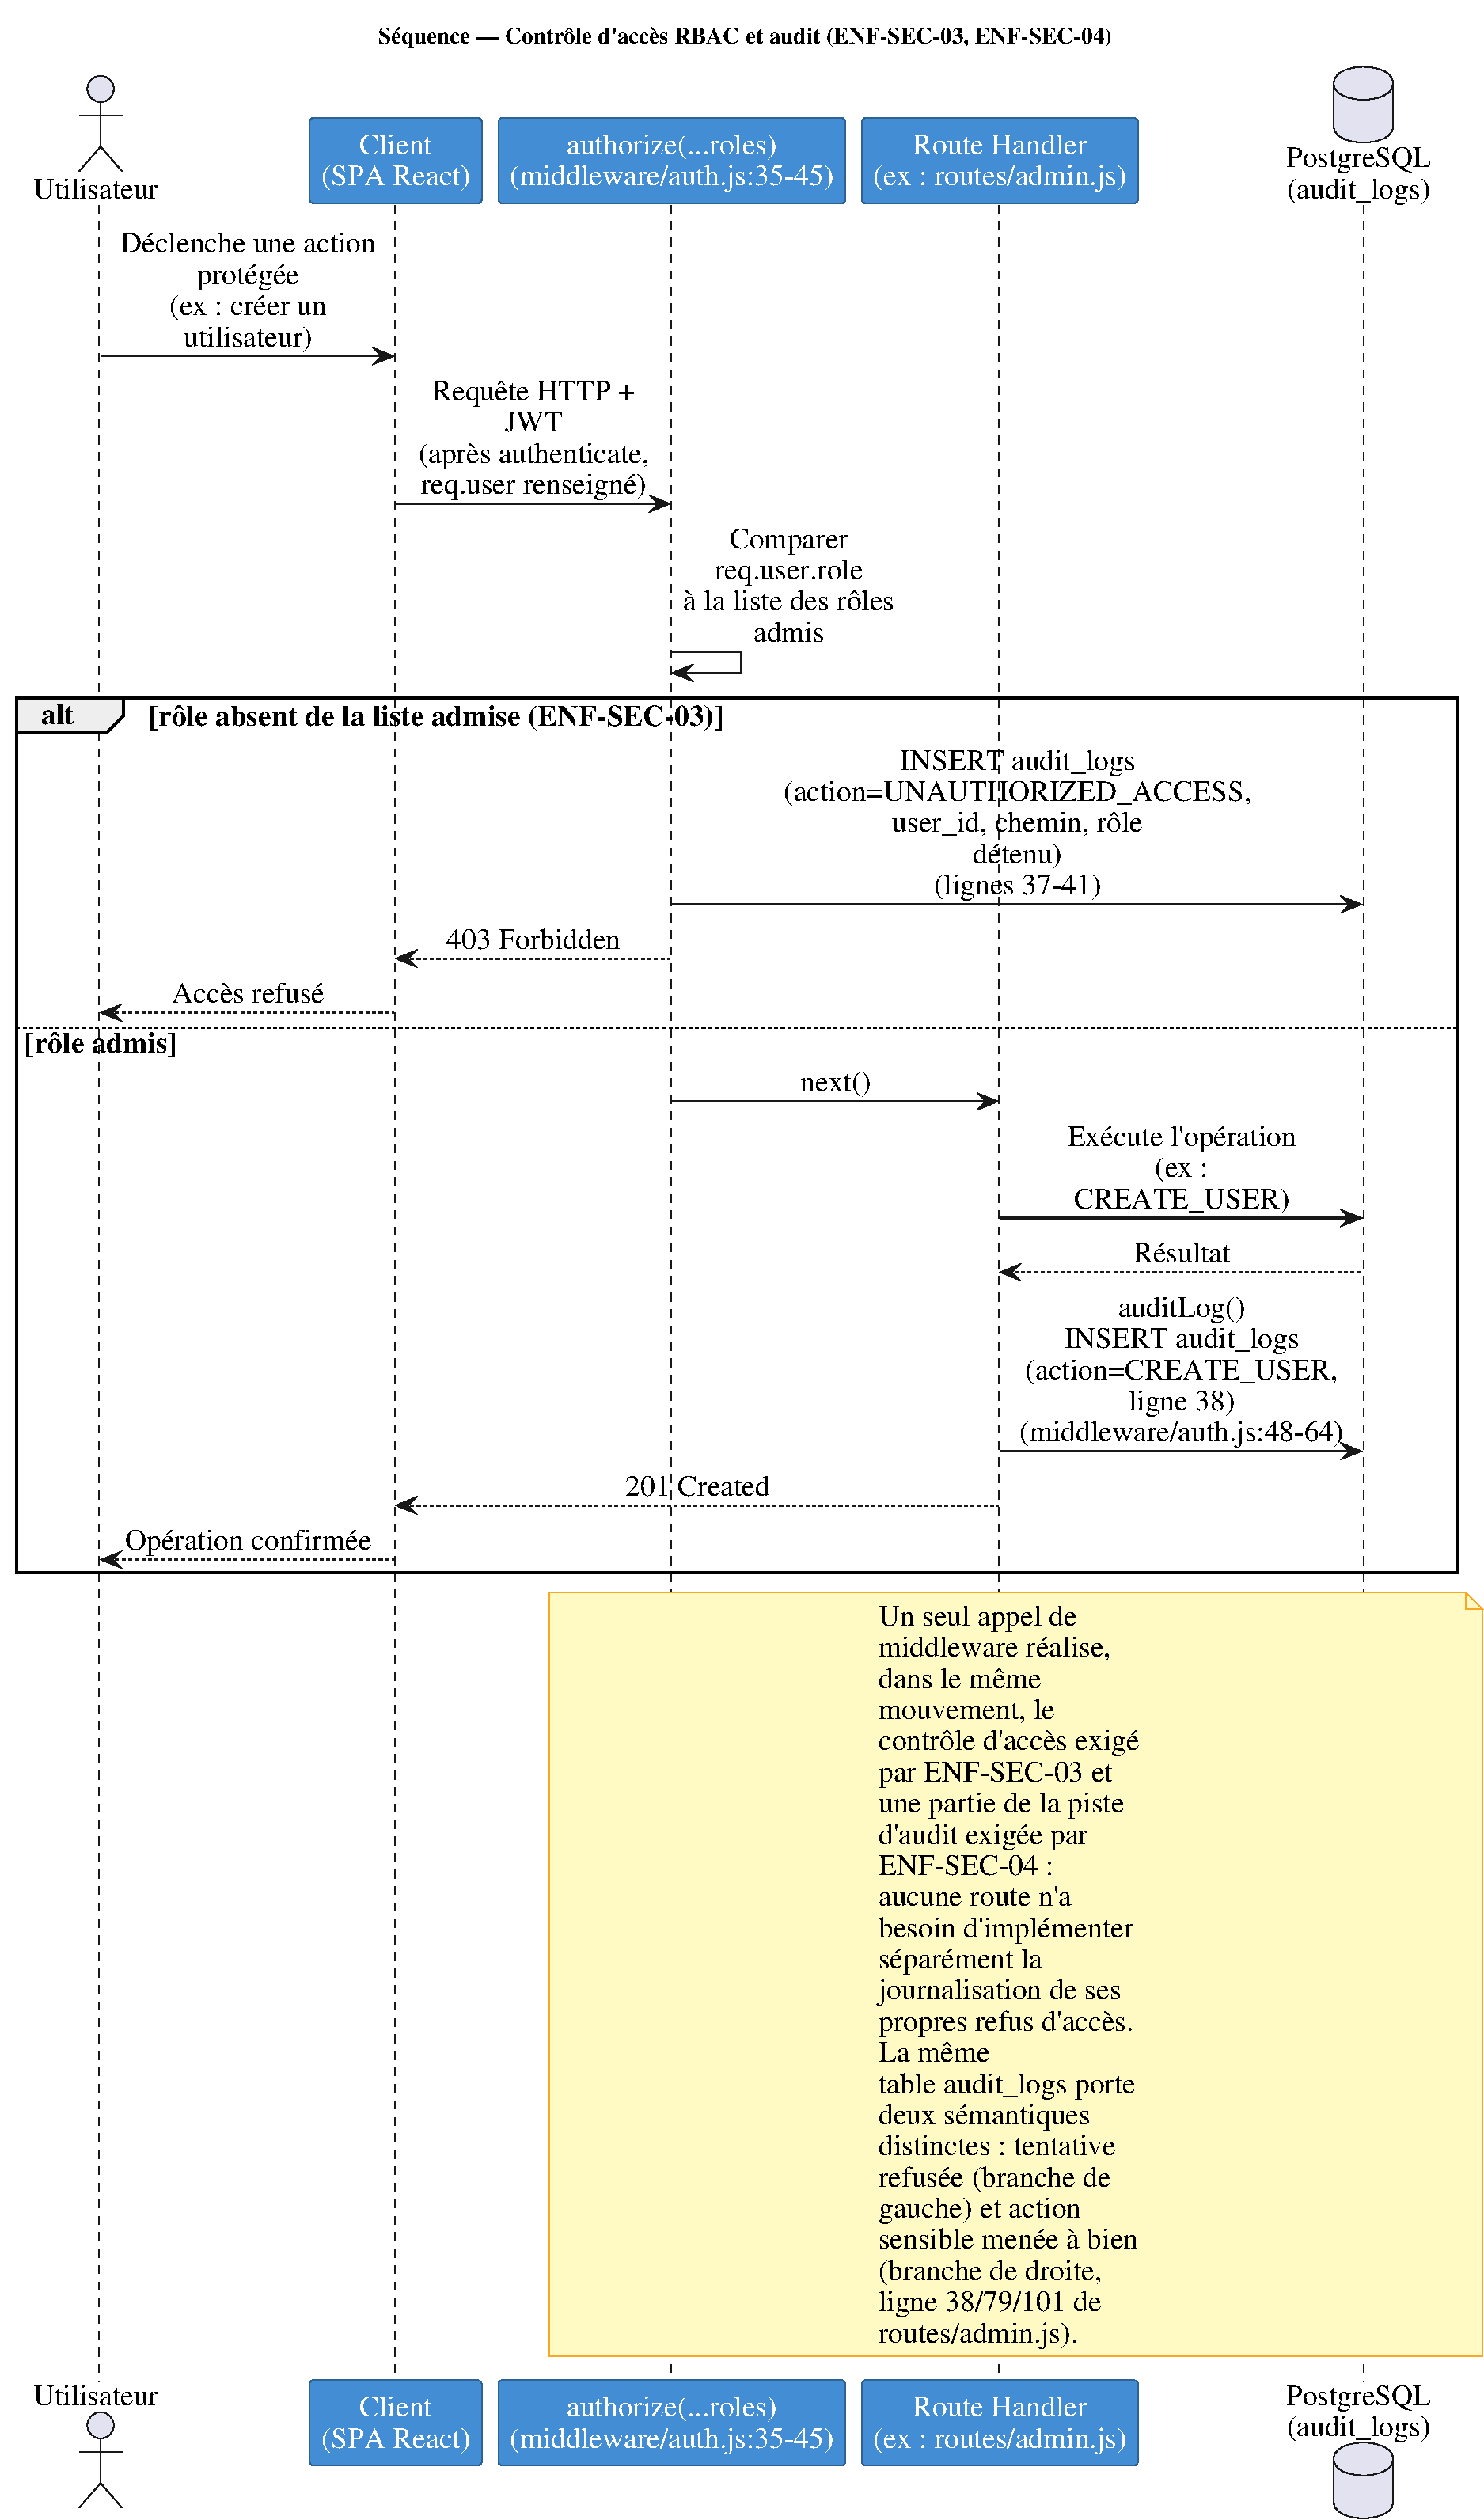
\includegraphics[width=\textwidth,height=0.88\textheight,keepaspectratio]{figures/fig_seq_rbac_audit.pdf}
    \caption{Séquence : contrôle d'accès RBAC et audit}
    \label{fig:seq_rbac_audit}
    \source{Schéma de l'auteur}
\end{figure}

\subsection{Reporting et export}
\label{sec:webapp_reporting}

Les récapitulatifs journalier et mensuel (\texttt{EF-REP-01}, \texttt{EF-REP-02}) et la recherche par période, camion ou catégorie (\texttt{EF-REP-04}) sont déployés. La Figure~\ref{fig:web_rapport} montre le rapport de juillet~2026 : totaux, solde de fin de mois, répartition des dépenses, classement des camions et détail chronologique.

\begin{figure}[H]
    \centering
    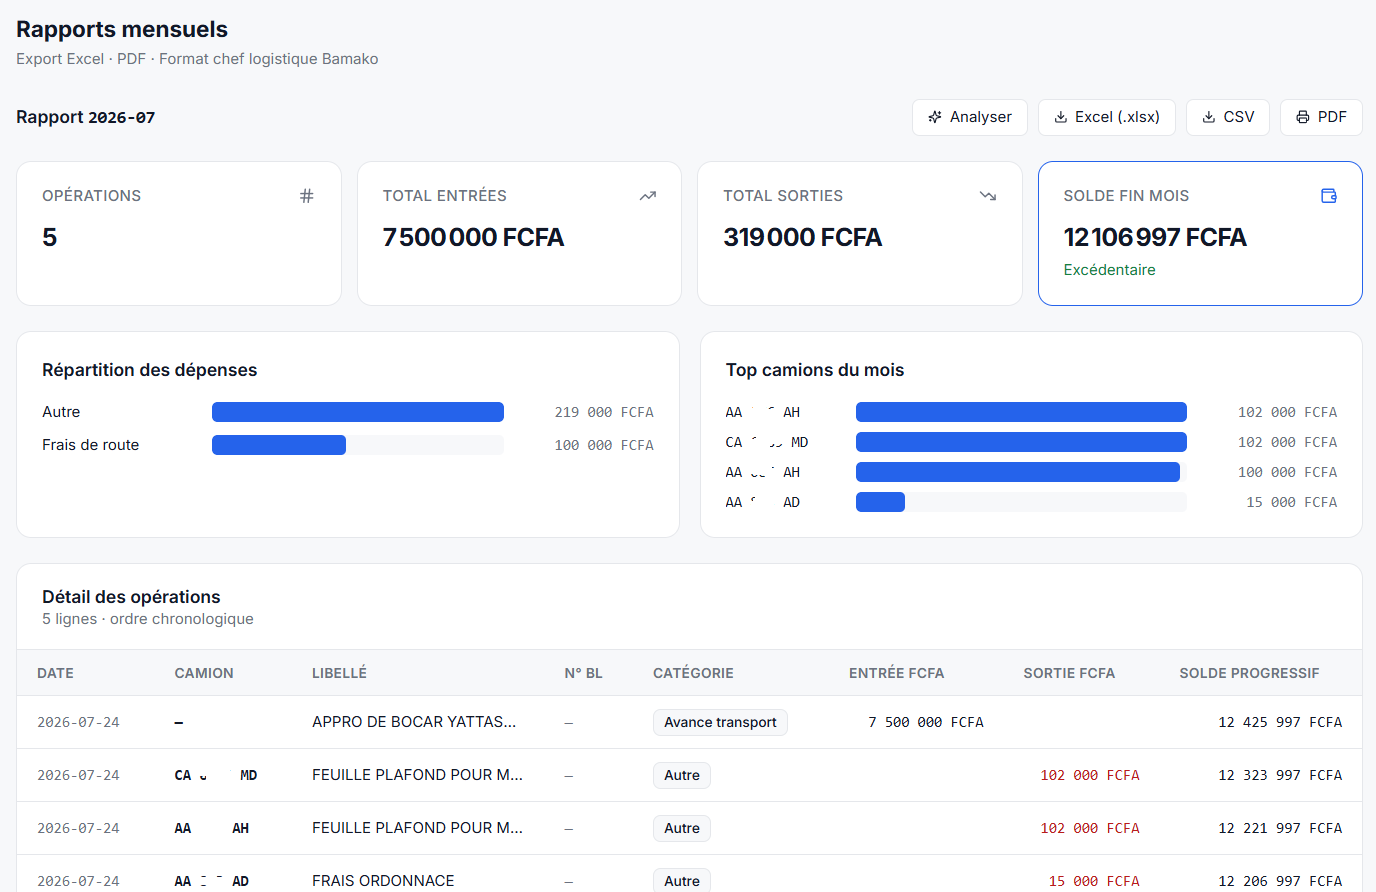
\includegraphics[width=0.75\textwidth]{figures/captures/web_rapport.png}
    \caption{Rapport mensuel consolidé (juillet~2026)}
    \label{fig:web_rapport}
\end{figure}

L'export (\texttt{EF-REP-03}) est partiel. Le CSV respecte l'usage français (encodage UTF-8 avec BOM, séparateur point-virgule) et s'ouvre directement dans Excel. Le fichier Excel est construit par le serveur, avec une feuille de résumé et une feuille de détail (Figure~\ref{fig:web_export}). Le bouton « PDF », en revanche, lance seulement l'impression du navigateur : aucun PDF n'est produit par le serveur. Un vrai export PDF est renvoyé aux perspectives.

\begin{figure}[H]
    \centering
    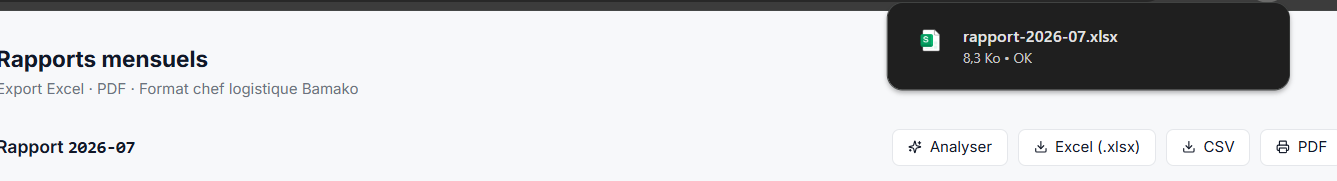
\includegraphics[width=0.8\textwidth]{figures/captures/web_export_xlsx.png}
    \caption{Export Excel du rapport mensuel : fichier \texttt{rapport-2026-07.xlsx} généré par le serveur}
    \label{fig:web_export}
\end{figure}

\subsection{Fonctionnalités cibles non déployées}
\label{sec:webapp_fonctionnalites_cibles_non_deployees}

\textbf{EF-VAL-02 : workflow de validation.} Chaque opération est enregistrée directement et définitivement : il n'existe ni statut (brouillon, validé), ni circuit d'approbation. Le visa manuscrit reste la référence pendant la transition, choix de priorité déjà justifié à la section~\ref{chap:besoins} (\S\ref{sec:synthese_tracabilite}) et représenté par le diagramme d'activité cible (Figure~\ref{fig:activite_validation_cible}).

\textbf{ENF-DISP-01 : mode hors-ligne.} Aucun mécanisme de saisie hors connexion n'existe : c'est une cible non entamée.

Ces deux manques ne remettent en cause ni la fin de la double saisie ni la visibilité en temps réel, déjà obtenues. Leur priorisation est discutée à la section~\ref{chap:discussion}.

\subsection{Synthèse et transition}
\label{sec:webapp_synthese_transition}

L'application réalise le cœur du cahier des charges : saisie unique et contrôlée, solde calculé par la base, accès cloisonné par rôle avec piste d'audit, rapports et exports. Elle reste une exploitation structurée, par formulaires et filtres. L'interrogation des données en langage naturel fait l'objet de la section suivante.

\section{Module d'IA générative hybride (RAG local et agent cloud)}
\label{chap:ia_rag}

Cette section décrit le module qui porte la contribution la plus distinctive de la plateforme : un agent conversationnel hybride, au sens défini en introduction. Un service local auto-hébergé (Mistral~7B via Ollama) traite les requêtes sensibles, qui doivent rester sous le contrôle de l'entreprise. Un service cloud (\texttt{claude-sonnet-4-5}, API Anthropic) traite les requêtes analytiques non sensibles, qui demandent une plus grande capacité de raisonnement. Nous décrivons ici la construction des deux chemins et du mécanisme qui les arbitre ; leur évaluation comparative, qui porte l'hypothèse H2, fait l'objet de la section~\ref{chap:benchmark_rag}.

\subsection{Architecture d'ensemble du module conversationnel hybride}
\label{sec:ia_archi}

Une requête suit toujours le même trajet. L'utilisateur la saisit dans le panneau conversationnel, ouvert par le bouton \textit{Assistant IA} de l'application (Figure~\ref{fig:ui_dashboard}). Un proxy de l'API Express la relaie à l'orchestrateur n8n, qui en évalue la sensibilité et la route vers l'un des deux chemins. L'échange est ensuite journalisé, quel que soit le chemin emprunté. Ce trajet est celui de la Figure~\ref{fig:seq_rag} (séquence) et de la Figure~\ref{fig:c4_conteneurs} (conteneurs) ; cette section en détaille l'implémentation.

\textbf{n8n comme point d'orchestration unique.} C'est le workflow n8n, et non l'application Express ou le service FastAPI, qui porte la logique hybride : il reçoit chaque requête, en évalue la sensibilité et décide du chemin (\texttt{EF-RAG-03}, ADR-02, \S\ref{sec:adr}). Les deux chemins augmentent la génération par des données métier réelles, mais par des mécanismes de récupération différents. Côté cloud (\S\ref{sec:ia_cloud}), un agent génère lui-même une requête SQL sur les vues relationnelles de la base. Côté local (\S\ref{sec:ia_local}), c'est le code du service qui récupère les données : par des filtres SQL déterministes (plaque, période, mots-clés) d'abord, par similarité vectorielle sur le corpus produit par l'ETL (\S\ref{sec:  vectorisation}) en dernier recours. Les deux relèvent du paradigme RAG au sens large : récupérer un contexte pertinent avant de générer.

\textbf{Le proxy Express.} Les routes qui relaient la requête vers n8n vivent dans le dépôt applicatif (section~\ref{chap:webapp}), mais relèvent de ce module. \texttt{POST~/api/chat} (\texttt{routes/chat.js}) est la route utilisée par le panneau conversationnel. Elle valide le message, le relaie au \textit{webhook} n8n avec un délai d'attente dimensionné pour les itérations d'un agent outillé, normalise la réponse et journalise l'échange dans \texttt{chat\_messages} (\S\ref{sec:ia_tracabilite}). Elle transmet aussi au client le chemin emprunté (\texttt{local} ou \texttt{cloud}), que l'interface affiche sous chaque réponse. \texttt{GET~/api/chat/history} expose l'historique d'un utilisateur. La route \texttt{POST~/api/analyze} (\texttt{index.js}) relaie elle aussi vers n8n, mais aucun composant du frontend ne l'appelle : c'est du code mort, que nous signalons comme tel.

\subsection{Le service RAG local souverain}
\label{sec:ia_local}

Le service FastAPI du chemin local est celui qui incarne le plus directement la souveraineté visée par H2 : un RAG conversationnel sur un corpus métier français, sans dépendance à un service tiers. Nous l'avons construit selon le schéma \textit{retriever--augmentation--generator} de Lewis et al. \cite{lewisRetrievalaugmentedGenerationKnowledgeintensive2020} (\S\ref{sec:Systemes_RAG_IA_Generative}), adapté à un corpus structuré et très redondant.

\subsubsection{Le retrieval : SQL exact d'abord, vectoriel en dernier recours}

\texttt{fetch\_rows()} applique une stratégie par passes successives. Elle repose sur une hypothèse simple : une correspondance exacte sur un identifiant métier (une plaque, une période, un mot du domaine) est un signal plus fiable qu'une similarité sémantique.

\begin{itemize}
    \item \textbf{Passe~0, la plaque.} Une immatriculation détectée dans la question filtre la vue \texttt{v\_transactions\_completes} sur la colonne \texttt{camion}, éventuellement croisée avec la période. Elle est prioritaire et isolée des autres mots-clés, pour ne pas diluer ce signal fort (« CAMION » figure dans des centaines de libellés sans rapport avec le véhicule visé).
    \item \textbf{Passes~1 et~2, les mots-clés.} Vingt et un mots déclencheurs du domaine (\textit{ex.} \texttt{CARBURANT}, \texttt{VIDANGE}, \texttt{RATION}) sont cherchés dans les libellés, d'abord en conjonction stricte, puis en disjonction. Certains sont traduits vers le vocabulaire réel de la base : « amende » ne figure dans aucun libellé, ce sont « contravention », « pesage » ou « défaut de papier » qui y figurent.
    \item \textbf{Filtres transverses.} Une période exprimée en toutes lettres (« mars 2026 », « T1 2026 ») ou au format ISO, et des critères de flotte (pays, type de propriété, statut) s'ajoutent en conjonction à toutes les passes. Si une question filtrée ne trouve rien, le service répond « aucune donnée » plutôt que de se replier sur une recherche vectorielle qui ignorerait le filtre.
    \item \textbf{Passe~3, le repli vectoriel.} Seulement si tout le reste échoue : la question est encodée par le même modèle qu'à l'ingestion (\texttt{all-MiniLM-L6-v2} \cite{reimersSentencebertSentenceEmbeddings2019}), puis comparée à \texttt{transport\_embeddings} par similarité cosinus (opérateur \texttt{<=>} de \texttt{pgvector}), qui renvoie les $k=10$ passages les plus proches \cite{karpukhinDensePassageRetrieval2020}.
\end{itemize}

\begin{lstlisting}[language=SQL, basicstyle=\ttfamily\footnotesize, breaklines=true, showstringspaces=false]
SELECT date, libelle, sortie FROM transport_embeddings
ORDER BY embedding <=> %s::vector ASC LIMIT 10
\end{lstlisting}

\textbf{Des réponses exactes sans modèle de langage.} Les LLM sont peu fiables en arithmétique. Nous avons donc retiré au modèle tout calcul qu'une requête SQL peut faire. Pour les passes~0 à~2, le total et le nombre d'opérations sont calculés par \texttt{SUM} et \texttt{COUNT} sur \emph{toutes} les lignes qui correspondent au filtre, pas seulement sur les dix transmises au modèle. Trois familles de questions sont ensuite servies directement, sans appel au LLM :
\begin{itemize}
    \item les comptages de camions (« combien de camions maliens actifs ? »), par un \texttt{COUNT} SQL ;
    \item le solde de caisse, calculé selon la même définition que la carte « Solde actuel » du tableau de bord ;
    \item les demandes d'agrégat (« total », « somme », « combien »), qui reçoivent le total SQL déjà calculé.
\end{itemize}
Pour les autres questions, le total est placé en tête du contexte, avec la mention « TOTAL EXACT (déjà calculé, à recopier tel quel) ». Pour le repli vectoriel, qui n'a pas de filtre exploitable, la mention devient « TOTAL APPROXIMATIF ». La part des questions du benchmark servies sans LLM est mesurée à la section~\ref{chap:benchmark_rag}.

\subsubsection{La génération}

Les questions ouvertes sont transmises à Mistral~7B par l'API de conversation d'Ollama (\texttt{http://ollama:11434/api/chat}), sous forme d'un message système et d'un message utilisateur contenant le contexte. Le message système impose une réponse en français de trois ou quatre phrases, la recopie mot pour mot du total fourni, la citation de deux ou trois postes de dépense représentatifs et l'aveu explicite d'une information absente. Nous avons fixé la température à~0,1, pour des réponses stables d'un appel à l'autre, et limité la sortie à 300~jetons. Le nom du modèle (\texttt{mistral:latest}) est écrit en dur dans la requête, et le message système est dupliqué entre les deux fonctions de génération : deux dettes de maintenabilité (\texttt{ENF-MAINT-01}, \texttt{ENF-MAINT-02}) reprises au §\ref{sec:ia_dettes}.

\subsubsection{Les points d'entrée}

Le service expose deux \textit{endpoints}, authentifiés par l'en-tête \texttt{X-API-Key} : \texttt{POST~/ask} renvoie la réponse complète en un bloc JSON ; \texttt{POST~/ask/stream} la restitue jeton par jeton. Le streaming répond à une contrainte d'usage : sans accélération matérielle (ADR-03, \S\ref{sec:adr}), l'inférence est lente, et une réponse qui se construit progressivement vaut mieux qu'un long silence. Un \textit{endpoint} \texttt{/health}, public et sans donnée, sert au contrôle de santé du conteneur (Figure~\ref{fig:ia_rag_api_logs}).

\begin{figure}[H]
    \centering
    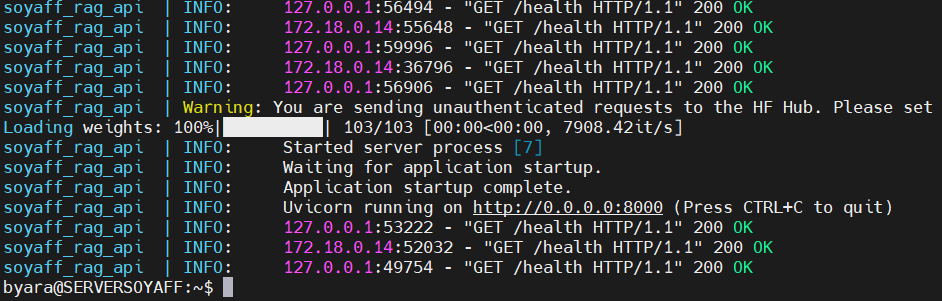
\includegraphics[width=0.65\textwidth]{figures/captures/ia_rag_api_logs.png}
    \caption{Démarrage du service RAG local en production et sondes de santé périodiques}
    \label{fig:ia_rag_api_logs}
\end{figure}

\textbf{Souveraineté par construction.} Sur ce chemin, aucune donnée de la base ne sort du serveur : le \textit{retrieval} interroge PostgreSQL en local, l'inférence s'exécute dans le conteneur Ollama du même réseau Docker, et seule la réponse finale est renvoyée à n8n. Cette étanchéité réalise \texttt{ENF-SOUV-01} pour ce chemin ; c'est un fait de construction, pas encore une mesure.

\subsection{Le chemin cloud}
\label{sec:ia_cloud}

Le second chemin traite les requêtes analytiques non sensibles (\texttt{EF-RAG-01}, \texttt{EF-RAG-02}) : agrégations, comparaisons temporelles, classements sur l'ensemble du référentiel. Pour ces requêtes, la capacité de raisonnement d'un grand modèle l'emporte sur la contrainte de souveraineté (\S\ref{sec:Systemes_RAG_IA_Generative}).

\textbf{Le modèle et son emplacement.} Le modèle est \texttt{claude-sonnet-4-5-}\allowbreak\texttt{20250929} de l'API Anthropic. L'appel n'est fait nulle part dans le code Express : il est porté par un nœud \textit{AI Agent} de n8n (\textit{framework} LangChain), connecté à un nœud de modèle Anthropic. Le proxy applicatif ignore l'existence de ce modèle.

\begin{sloppypar}
\textbf{Un agent outillé.} L'agent dispose d'un outil d'exécution SQL sur PostgreSQL. La requête est générée par le modèle à partir d'un \textit{system prompt} versionné (\texttt{n8n/system\_prompt\_agent.md}), qui documente les vues métier (\texttt{v\_transactions\_completes}, \texttt{v\_stats\_par\_camion}, \texttt{v\_resume\_mensuel}, \texttt{v\_stats\_par\_produit}), les conventions du domaine et des exemples de correspondance question--requête. Une mémoire conversationnelle, également dans PostgreSQL, conserve les dix derniers échanges d'une session : l'agent peut ainsi résoudre « ce camion » dans une question de relance. La réponse suit un gabarit imposé : tableau, analyse, recommandation le cas échéant.
\end{sloppypar}

\textbf{Un accès en lecture seule.} Le SQL généré par un modèle ne doit pas pouvoir modifier la base. Nous avons donc connecté l'outil SQL à un rôle PostgreSQL dédié, \texttt{soyaff\_agent\_ro} (migration Alembic~004). Ses sessions sont en lecture seule par défaut, ses requêtes sont interrompues au-delà de 15~secondes et il ne peut ouvrir que cinq connexions. Il ne lit que les tables et vues métier ; la table \texttt{chauffeurs} (noms, téléphones), les embeddings et l'historique des conversations lui sont inaccessibles. La mémoire de conversation utilise un autre compte. La garantie ne repose donc plus sur l'obéissance du modèle aux consignes, mais sur les droits de la base (voir le test du §\ref{sec:test_bout_en_bout}).

\textbf{Une frontière franchie.} Ce chemin traverse le périmètre souverain de la Figure~\ref{fig:c4_conteneurs} : la question de l'utilisateur et les résultats des requêtes SQL de l'agent sont traités par un service tiers. Le routage décrit ci-dessous existe pour limiter ce franchissement aux requêtes non sensibles.

\subsection{Le routage par sensibilité}
\label{sec:ia_routage}

Le routage est le mécanisme qui fait exister l'hybride au sens de l'introduction ; il réalise \texttt{EF-RAG-03}. Chaque requête entre dans le workflow n8n de la Figure~\ref{fig:ia_workflow}, dont le premier nœud de code en évalue la sensibilité. Une requête sensible part vers le service local par une requête HTTP authentifiée (\texttt{POST~http://api:8000/ask}) ; une requête non sensible est confiée à l'agent cloud. Nous avons formalisé cette décision dans l'\texttt{ADR-02} (\S\ref{sec:adr}) : un point de décision unique plutôt qu'une logique dispersée dans chaque service.

\begin{figure}[H]
    \centering
    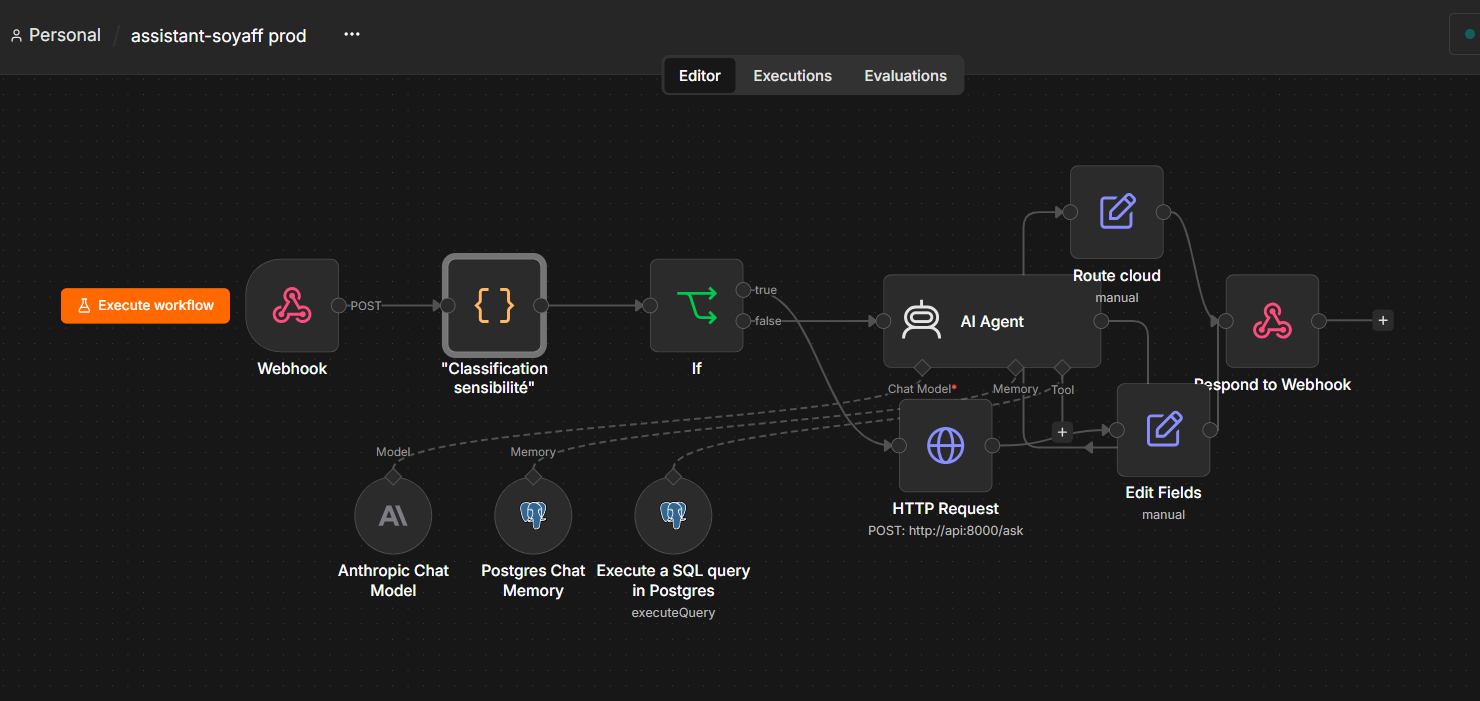
\includegraphics[width=0.85\textwidth]{figures/captures/ia_workflow_n8n.png}
    \caption{Workflow n8n de routage hybride en production}
    \label{fig:ia_workflow}
\end{figure}

\textbf{Le mécanisme.} La classification est une heuristique par mots entiers et expressions régulières, appliquée à la question débarrassée de ses accents et mise en majuscules (Figure~\ref{fig:ia_classifieur}). Ce n'est pas un classifieur d'apprentissage automatique, ainsi que l'assume l'\texttt{ADR-02}. Deux règles décident :
\begin{itemize}
    \item toute mention d'\textbf{identité} reste locale, même dans une question d'agrégat : un terme comme \textit{chauffeur}, \textit{salaire}, \textit{paie}, \textit{téléphone}, \textit{CNI} ou \textit{adresse}, ou une plaque d'immatriculation (« total du camion AA~076~AH », « top des chauffeurs ») ;
    \item un \textbf{montant financier précis} (\textit{solde}, \textit{reliquat}, \textit{avance}, « combien doit ») reste local, \emph{sauf} si la question est explicitement agrégée (\textit{total}, \textit{moyenne}, \textit{comparaison}, \textit{tendance}, \textit{top}, \textit{classement}, \textit{évolution}, pourcentage).
\end{itemize}
La seconde règle traduit un choix assumé : tout le métier de SOYAFF est financier, et classer sensible toute mention de montant viderait le chemin cloud de son utilité. La recherche par mot entier évite les faux déclencheurs (« TOP » dans « STOP », « PAIE » dans « PAIEMENT »), et le motif de plaque écarte les faux positifs du français courant (« EN 2025 », « DE 1500 »).

\begin{figure}[H]
    \centering
    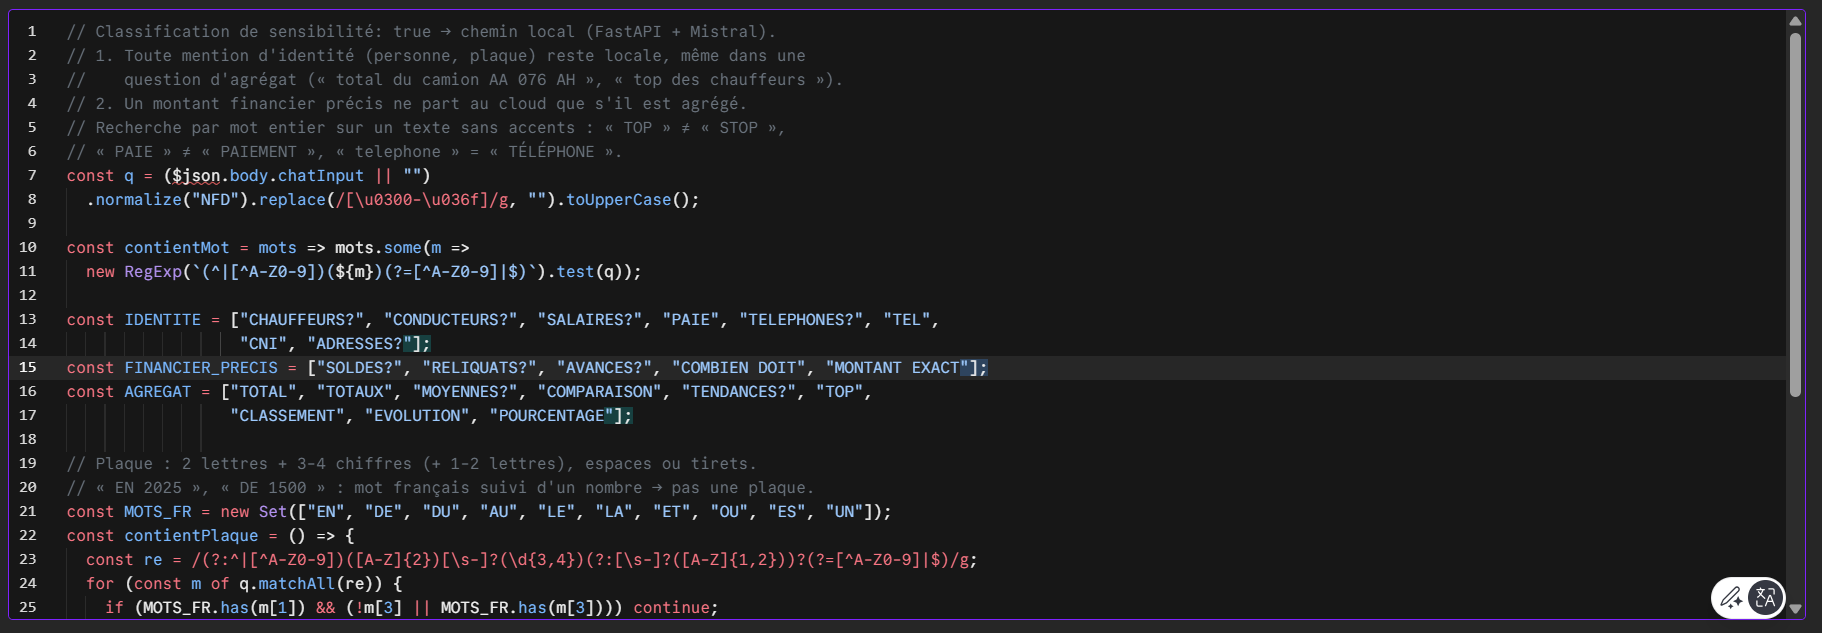
\includegraphics[width=0.9\textwidth]{figures/captures/ia_classifieur.png}
    \caption{Règles du classifieur de sensibilité (nœud de code n8n, extrait)}
    \label{fig:ia_classifieur}
\end{figure}

\textbf{Le routage vérifié.} Les Figures~\ref{fig:ia_route_locale} et~\ref{fig:ia_route_cloud} montrent les deux chemins en production. Une question sur les dépenses d'un camion identifié est traitée en local : la réponse est un total SQL exact, sans appel au LLM. Une question agrégée sur la flotte est traitée par l'agent cloud, qui répond par un tableau, une analyse et des recommandations. L'étiquette affichée sous chaque réponse indique le chemin emprunté, jamais le modèle utilisé.

\begin{figure}[H]
    \centering
    \begin{minipage}[t]{0.48\textwidth}
        \centering
        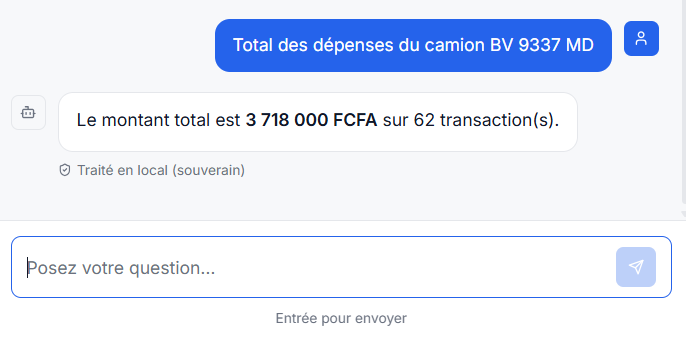
\includegraphics[width=\textwidth]{figures/captures/ia_route_locale.png}
        \caption{Question portant sur un camion identifié : traitée en local (souverain)}
        \label{fig:ia_route_locale}
    \end{minipage}\hfill
    \begin{minipage}[t]{0.48\textwidth}
        \centering
        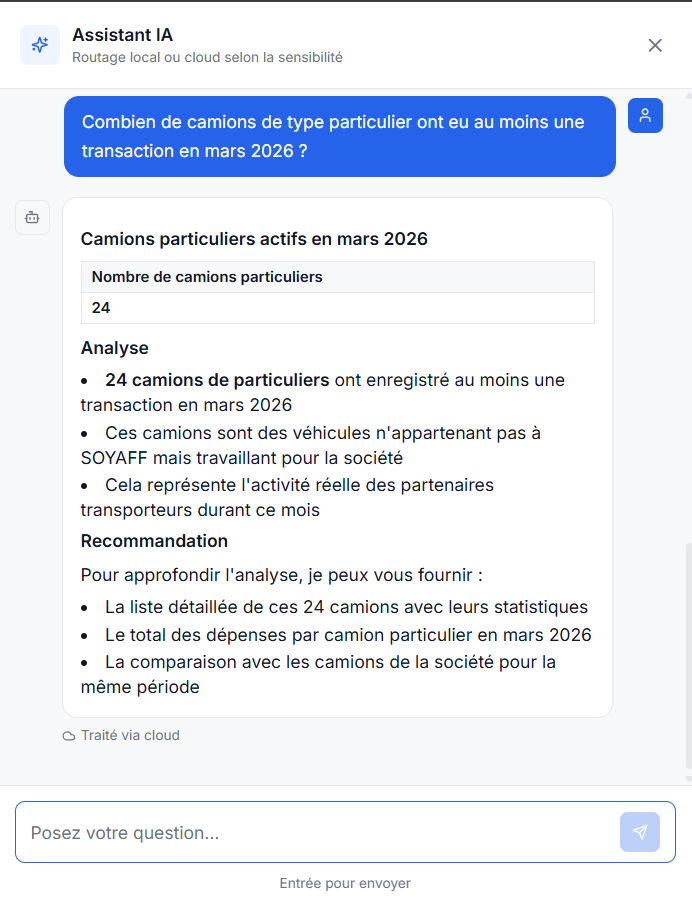
\includegraphics[width=\textwidth]{figures/captures/ia_route_cloud.png}
        \caption{Question agrégée sur la flotte : traitée via le cloud}
        \label{fig:ia_route_cloud}
    \end{minipage}
\end{figure}

\textbf{Une limite résiduelle.} L'heuristique reste lexicale. Un nom de chauffeur cité seul, sans le mot « chauffeur » ni plaque, n'est pas détecté : la requête part vers le cloud. Le risque est borné par le rôle en lecture seule (\S\ref{sec:ia_cloud}) : l'agent n'a pas accès à la table \texttt{chauffeurs} et ne peut donc pas associer ce nom à des données personnelles. Le workflow est versionné dans le dépôt \texttt{assistant-soyaff-1} (\texttt{n8n/assistant-soyaff-hybrid-routing.json}) : la classification, les deux branches et leur authentification sont reproductibles indépendamment de l'instance n8n en production.

\textbf{La conséquence méthodologique.} L'hypothèse H2 porte sur la parité d'exactitude entre les deux \emph{services d'inférence}, pas sur la justesse du classifieur qui choisit entre eux. Mesurer H2 à travers le chemin réellement emprunté par n8n ferait dépendre le résultat de la précision du classifieur, une autre question. Le benchmark de la section~\ref{chap:benchmark_rag} interroge donc chaque service directement, sur le même jeu de questions. La validité du classifieur est un chantier d'évaluation distinct, non couvert par H2.

\subsection{Citation des sources et journalisation}
\label{sec:ia_tracabilite}

\textbf{Citation des sources (EF-RAG-04) : une transparence sur le contexte.} Le service local renvoie, à côté de la réponse, les lignes qui ont servi à la construire (date, libellé, montant) et le total exact : dans le champ \texttt{context} de \texttt{/ask}, et dans l'en-tête \texttt{X-RAG-Context} de \texttt{/ask/stream}. C'est une transparence sur le contexte, pas une citation au sens strict : aucune affirmation du texte généré n'est reliée à un enregistrement précis. Côté cloud, le \textit{system prompt} ne demande pas de citation ; le tableau que l'agent inclut dans sa réponse montre les lignes renvoyées par sa requête SQL, sans mécanisme de citation formalisé. \texttt{EF-RAG-04} est donc partiellement réalisée.

\textbf{Journalisation (EF-RAG-05) : uniforme, en aval du routage.} Chaque échange est consigné dans \texttt{chat\_messages} (\texttt{user\_id}, \texttt{role}, \texttt{content}, \texttt{created\_at}) par le proxy Express : le message de l'utilisateur, puis la réponse, quel que soit le chemin qui l'a produite. Cette journalisation sert la piste d'audit exigée par \texttt{ENF-SEC-04} et constitue un corpus de questions réelles utile à l'évaluation. La mémoire conversationnelle de l'agent cloud (\S\ref{sec:ia_cloud}) est un mécanisme distinct : elle sert la continuité d'une session, sans les métadonnées d'audit ni l'exhaustivité exigées par \texttt{EF-RAG-05}.

\subsection{Écarts, dettes et cohérence}
\label{sec:ia_dettes}

Nous rassemblons ici les écarts du volet IA ; leur priorisation est discutée à la section~\ref{chap:discussion}. Ce sont des dettes de finition et de traçabilité, pas des défauts des moteurs d'inférence : les deux chemins existent, répondent et sont arbitrés par le routage.

\begin{itemize}
    \item \textbf{\texttt{ENF-MAINT-01} : pas d'interface d'inférence abstraite.} Le nom du modèle local est écrit en dur dans l'appel à Ollama ; changer de modèle impose de modifier le code.
    \item \textbf{\texttt{ENF-MAINT-02} : message système dupliqué} entre les fonctions de génération bloquante et en flux, au lieu d'être factorisé.
    \item \textbf{Citation des sources partielle (\texttt{EF-RAG-04}).} Transparence sur le contexte côté local, aucune citation structurée des enregistrements sur l'un ou l'autre chemin.
    \item \textbf{Classifieur lexical (\texttt{EF-RAG-03}).} Un nom de chauffeur cité seul n'est pas détecté ; le rôle en lecture seule borne le risque sans le supprimer.
\end{itemize}

Plusieurs dettes relevées lors de la première rédaction ont été refermées depuis. L'outil SQL de l'agent cloud n'avait aucun garde-fou technique : il utilise désormais le rôle \texttt{soyaff\_agent\_ro}. Le classifieur envoyait au cloud une question d'agrégat nommant un chauffeur ou un camion : l'identité l'emporte désormais sur l'agrégat. Le total transmis au modèle local ne sommait que les dix lignes affichées : il est calculé en SQL sur toutes les lignes correspondantes. Enfin, le contexte n'était pas exposé en mode streaming : il l'est par l'en-tête \texttt{X-RAG-Context}. L'\texttt{ADR-02} (\S\ref{sec:adr}) signale ces résorptions.

\subsection{Synthèse et transition}

Nous avons construit dans cette section les deux chemins de l'agent conversationnel hybride et le mécanisme qui les arbitre. Le service local (\S\ref{sec:ia_local}) réalise par construction la souveraineté d'\texttt{ENF-SOUV-01} et ne confie au modèle de langage que ce qu'une requête SQL ne sait pas faire. Le chemin cloud (\S\ref{sec:ia_cloud}) s'appuie sur un agent outillé, borné par un rôle en lecture seule. Le routage (\S\ref{sec:ia_routage}) a été vérifié dans les deux sens en production, et le workflow qui le porte est versionné. Nous n'avançons ici aucun chiffre de performance : cette mesure est l'objet de la section~\ref{chap:benchmark_rag}.

Ces modules ne tiennent en production que parce qu'une infrastructure les déploie, les supervise et les maintient disponibles avec des ressources limitées. C'est l'objet de la section suivante.

\section{Infrastructure DevOps et observabilité}
\label{chap:devops}

Cette section décrit la couche qui déploie, teste en continu et supervise les services présentés aux sections~\ref{chap:etl}, \ref{chap:webapp} et~\ref{chap:ia_rag}. Elle pose les conditions matérielles de l'hypothèse de frugalité H1 (\texttt{ENF-FRUG-01}) et réalise le volet infrastructure de \texttt{ENF-DISP-02} (disponibilité), \texttt{ENF-SEC-04}/\texttt{05} (audit, TLS), \texttt{ENF-MAINT-02} (tests en intégration continue) et \texttt{EF-ADM-03} (sauvegarde). Le chiffrage du coût réel et la validation de H1 relèvent de la section~\ref{chap:impact_metier}.

\subsection{Conteneurisation et déploiement mono-hôte}
\label{sec:devops_conteneurisation}

La vue de déploiement de la section~\ref{chap:architecture} (Figure~\ref{fig:deploiement}) situe l'infrastructure : tous les services tournent sur le serveur dédié décrit au §\ref{sec:env_realisation}, loué 30,23~USD par mois. Nous citons ce montant comme donnée de conception qui justifie le choix mono-hôte de l'ADR-03 (\S\ref{sec:adr}) ; sa confrontation au seuil de \texttt{ENF-FRUG-01}, avec les autres postes de coût, relève de la section~\ref{chap:impact_metier}.

Docker Engine orchestre l'ensemble sur un réseau unique, \texttt{soyaff\_network}. Chaque conteneur ne publie ses ports que sur \texttt{127.0.0.1} : ni la base PostgreSQL, ni l'API RAG, ni Airflow ne sont atteignables autrement que depuis le serveur lui-même. Quatorze conteneurs tournent en permanence, répartis en trois fichiers \texttt{docker compose} versionnés : la pile IA/ETL et la supervision dans le dépôt \texttt{assistant-soyaff}, l'application dans le dépôt \texttt{assistant-soyaff-app}. Le Tableau~\ref{tab:inventaire_conteneurs} les regroupe par plan fonctionnel.

\begin{table}[htbp]
\centering
\footnotesize
\caption{Inventaire des conteneurs de production, par plan fonctionnel (état au 27~septembre~2026)}
\label{tab:inventaire_conteneurs}
\begin{tabularx}{\linewidth}{|l|>{\raggedright\arraybackslash}p{5.5cm}|>{\raggedright\arraybackslash}X|}
\hline
\rowcolor[HTML]{EFEFEF}
\textbf{Plan} & \textbf{Conteneurs} & \textbf{Rôle} \\ \hline
Applicatif & \texttt{soyaff\_frontend}, \texttt{soyaff\_backend} & SPA React servie par un Nginx conteneurisé (\S\ref{sec:webapp_architecture}) ; API REST Express \\ \hline
Données & \texttt{soyaff\_postgres} & Moteur relationnel et vectoriel unique (PostgreSQL~16 + pgvector), mutualisé entre l'application, l'ETL et le RAG (ADR-04) \\ \hline
IA~/~RAG & \texttt{soyaff\_rag\_api}, \texttt{ollama} & Service FastAPI du chemin local (section~\ref{chap:ia_rag}) ; inférence Mistral~7B \\ \hline
ETL & \texttt{soyaff\_airflow\_web}, \texttt{airflow\_scheduler} & Interface et ordonnanceur du pipeline d'ingestion (section~\ref{chap:etl}, ADR-01) \\ \hline
Automatisation & \texttt{soyaff\_n8n} & Orchestrateur du routage hybride (ADR-02) \\ \hline
Supervision & \texttt{soyaff\_prometheus}, \texttt{soyaff\_node\_exporter}, \texttt{soyaff\_blackbox}, \texttt{soyaff\_loki}, \texttt{soyaff\_promtail}, \texttt{soyaff\_grafana} & Métriques et sondes (exportateurs~$\rightarrow$~Prometheus), journaux (Promtail~$\rightarrow$~Loki), tableaux de bord et alertes (Grafana), \S\ref{sec:devops_observabilite} \\ \hline
\end{tabularx}
\end{table}

Deux composants tournent hors de Docker. Un Nginx installé sur le serveur reçoit tout le trafic sur les ports~80 et~443 et le route par sous-domaine (\texttt{api.}, \texttt{n8n.}, \texttt{airflow.}, \texttt{monitor.soyaff-logstique.com}) vers le port local du conteneur concerné. Le \textit{runner} GitLab, service système, exécute les pipelines (\S\ref{sec:devops_cicd}). Le pare-feu \texttt{UFW} n'ouvre que les ports~22 (SSH), 80 et~443 (\S\ref{sec:devops_securite}).

Cette topologie mono-hôte, entièrement open source, rend la frugalité possible : c'est une \emph{condition} de H1, pas un résultat établi ici. Sa contrepartie est le point de défaillance unique assumé à l'ADR-03 : une panne du serveur arrête tous les services à la fois. Ce compromis est repris à la section~\ref{chap:discussion}.

\subsection{Intégration et déploiement continus (CI/CD GitLab)}
\label{sec:devops_cicd}

Les deux dépôts sont hébergés sur GitLab.com. Nous avons installé sur le serveur un \textit{runner} dédié, à \textit{executor} \texttt{shell}, qui exécute chaque job directement sur le serveur (Figure~\ref{fig:ops_runner}). C'est cohérent avec le mono-hôte de l'ADR-03 : les jobs de déploiement agissent sans intermédiaire sur les conteneurs de production. La contrepartie est qu'un job mal isolé pourrait, en principe, affecter le serveur lui-même.

\begin{figure}[H]
    \centering
    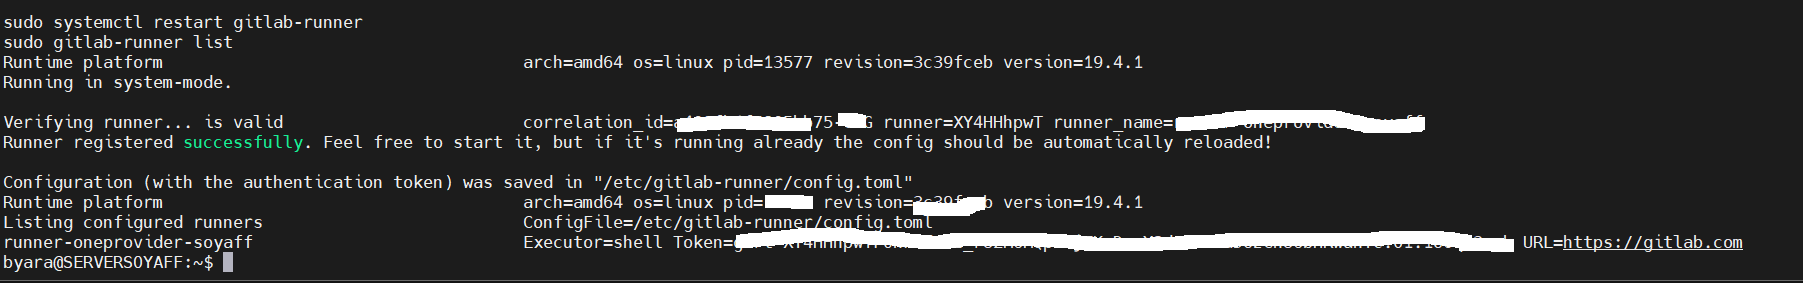
\includegraphics[width=0.9\textwidth]{figures/captures/ops_runner.png}
    \caption{Enregistrement du \textit{runner} GitLab sur le serveur de production}
    \label{fig:ops_runner}
\end{figure}

Deux dépôts, deux pipelines indépendants : \texttt{assistant-soyaff} porte la pile Python (ETL, RAG, supervision), \texttt{assistant-soyaff-app} l'application web. Leur ordre de déploiement est une contrainte opérationnelle : le second vérifie que le réseau \texttt{soyaff\_network}, créé par le premier, existe, et s'interrompt sinon.

\textbf{Des tests qui bloquent réellement.} Le Tableau~\ref{tab:cicd_jobs} détaille chaque job de test. Tous font échouer le pipeline en cas d'erreur, et un pipeline en échec ne déploie rien.

\begin{table}[htbp]
\centering
\footnotesize
\caption{Jobs de test des deux pipelines (état au 27~septembre~2026)}
\label{tab:cicd_jobs}
\begin{tabularx}{\linewidth}{|l|l|>{\raggedright\arraybackslash}X|>{\raggedright\arraybackslash}p{2.6cm}|}
\hline
\rowcolor[HTML]{EFEFEF}
\textbf{Job} & \textbf{Dépôt} & \textbf{Ce qu'il exécute} & \textbf{Couverture} \\ \hline
\texttt{test:python} & \texttt{assistant-soyaff} & Vérification de syntaxe des modules, puis \texttt{pytest} : 397 tests, dont des tests d'intégration contre un PostgreSQL~16 + pgvector jetable, démarré pour le job & 97,6~\% mesurés, plancher bloquant à 95~\% \\ \hline
\texttt{lint:backend}, \texttt{lint:frontend} & \texttt{assistant-soyaff-app} & ESLint et Prettier & sans objet \\ \hline
\texttt{test:backend} & \texttt{assistant-soyaff-app} & Jest : 122 tests unitaires et d'intégration contre une base de test & non mesurée en CI \\ \hline
\texttt{test:frontend} & \texttt{assistant-soyaff-app} & Vitest : 44 tests, puis construction de production & non mesurée en CI \\ \hline
\end{tabularx}
\end{table}

Les Figures~\ref{fig:ops_test_python}, \ref{fig:ops_test_backend} et~\ref{fig:ops_test_frontend} montrent ces trois suites en succès. Côté Python, nous avons fixé le plancher de couverture par cliquet : il est relevé à chaque progression mesurée, jamais abaissé.

\begin{figure}[H]
    \centering
    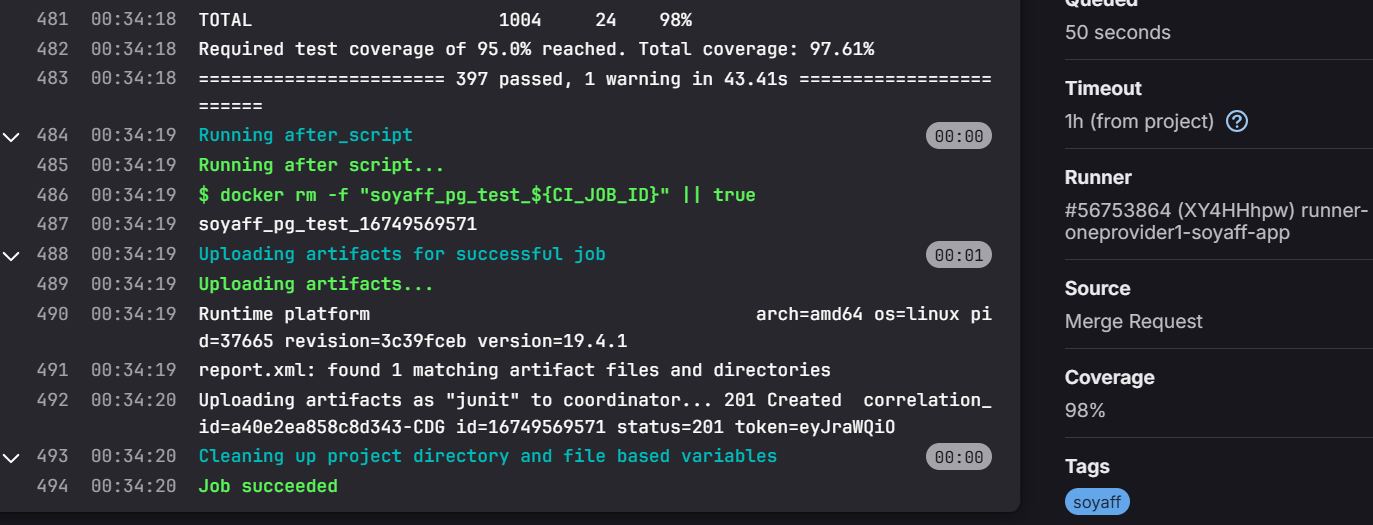
\includegraphics[width=0.7\textwidth]{figures/captures/ops_test_python.png}
    \caption{Job \texttt{test:python} : 397 tests réussis, couverture de 97,61~\% pour un plancher de 95~\%}
    \label{fig:ops_test_python}
\end{figure}

\begin{figure}[H]
    \centering
    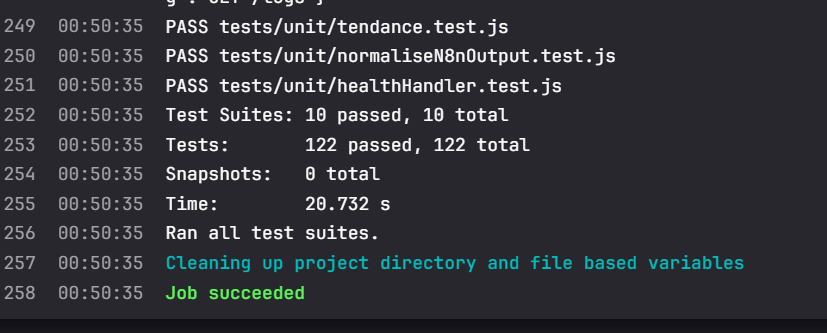
\includegraphics[width=0.5\textwidth]{figures/captures/ops_test_backend.png}
    \caption{Job \texttt{test:backend} : 122 tests réussis}
    \label{fig:ops_test_backend}
\end{figure}

\begin{figure}[H]
    \centering
    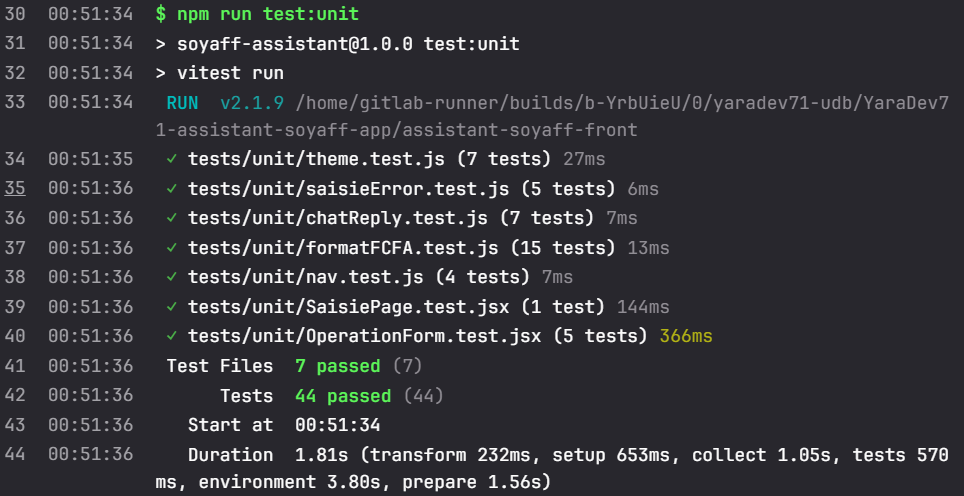
\includegraphics[width=0.55\textwidth]{figures/captures/ops_test_frontend.png}
    \caption{Job \texttt{test:frontend} : 44 tests réussis}
    \label{fig:ops_test_frontend}
\end{figure}

\textbf{Un déploiement automatique.} Les jobs \texttt{deploy:production} n'ont aucune validation manuelle : toute fusion sur \texttt{main} déploie. Le job récupère le code (\texttt{git reset --hard origin/main}), génère le fichier \texttt{.env} à partir des variables protégées de GitLab (aucun secret n'est écrit dans le dépôt), puis reconstruit et redémarre les conteneurs. Côté Python, il applique d'abord les migrations Alembic. Côté application, il interroge ensuite la sonde de santé du backend : si elle ne répond pas, le job échoue (Figure~\ref{fig:ops_deploy_app}). La Figure~\ref{fig:ops_pipelines} montre l'historique des pipelines : un job de test dure environ deux minutes et demie, un déploiement une trentaine de secondes.

\begin{figure}[H]
    \centering
    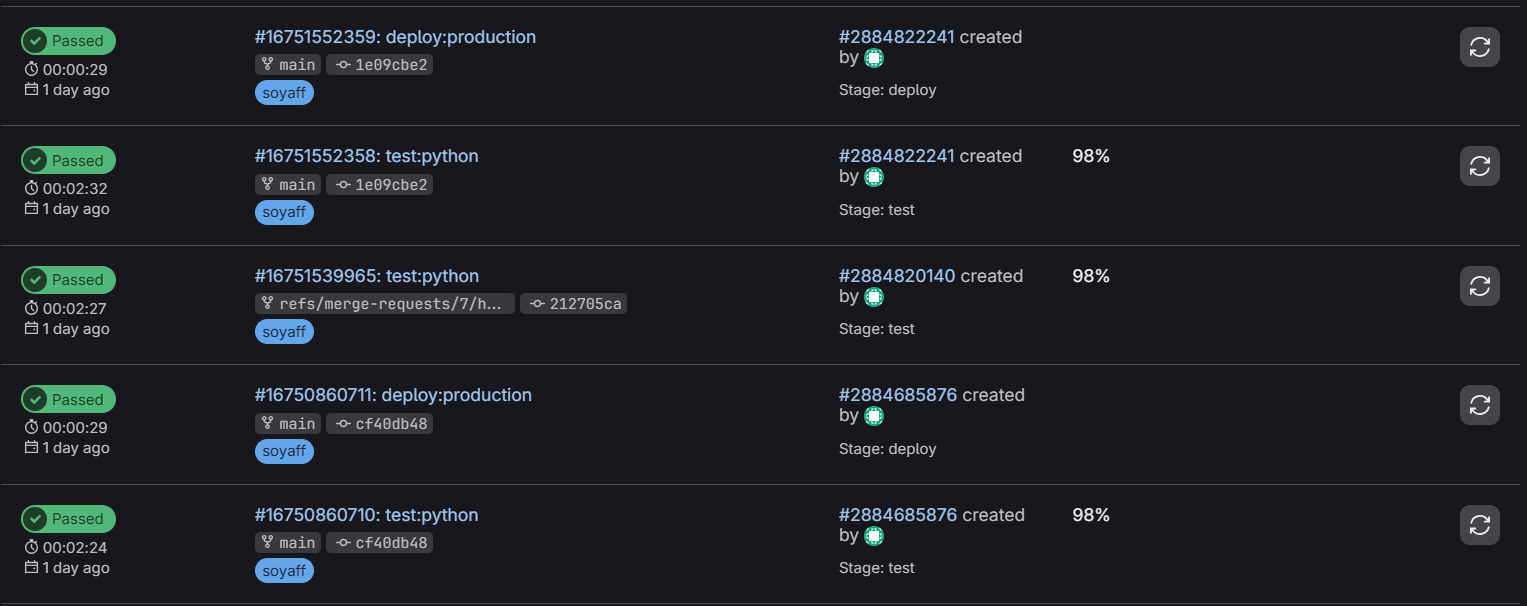
\includegraphics[width=0.85\textwidth]{figures/captures/ops_pipelines.png}
    \caption{Historique des jobs CI/CD : tests (couverture 98~\%) puis déploiement sur \texttt{main}}
    \label{fig:ops_pipelines}
\end{figure}

\begin{figure}[H]
    \centering
    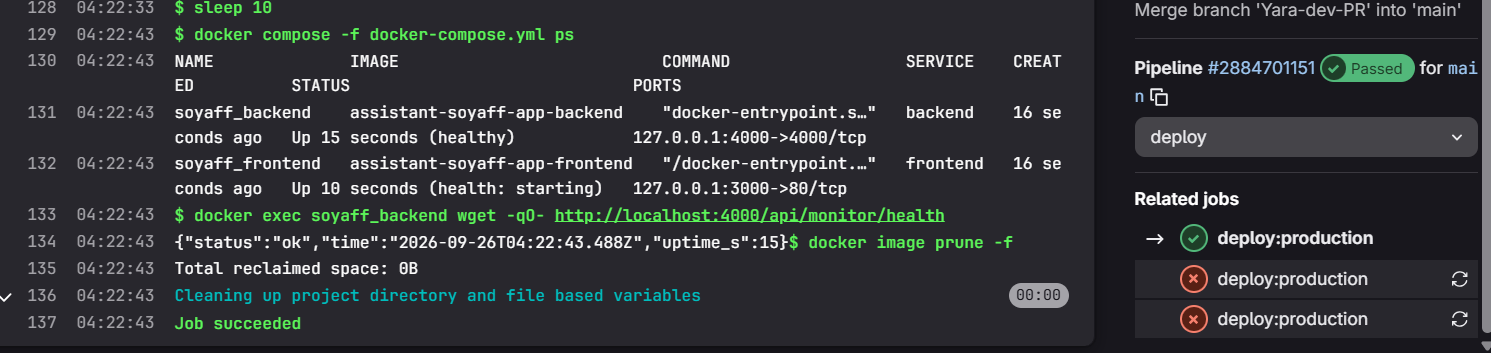
\includegraphics[width=0.85\textwidth]{figures/captures/ops_deploy_app.png}
    \caption{Déploiement automatique de l'application, vérifié par la sonde de santé du backend}
    \label{fig:ops_deploy_app}
\end{figure}

\begin{figure}[H]
    \centering
    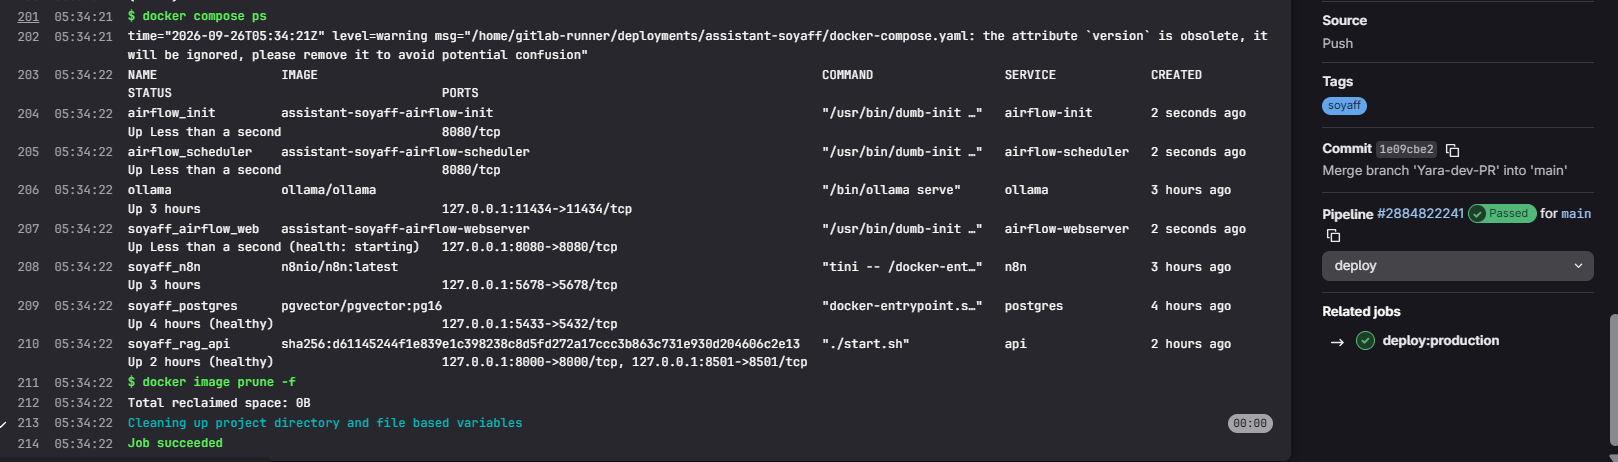
\includegraphics[width=0.85\textwidth]{figures/captures/ops_deploy_ia.png}
    \caption{Déploiement automatique de la pile IA/ETL : état des conteneurs en fin de job}
    \label{fig:ops_deploy_ia}
\end{figure}

Ce déploiement continu n'a pas de stratégie de bascule : ni \textit{blue-green}, ni retour arrière automatique. Côté Python, l'état des conteneurs affiché en fin de job (Figure~\ref{fig:ops_deploy_ia}) est informatif et ne fait pas échouer le job. Cette dette est reprise au \S\ref{sec:devops_dettes}.

\textbf{La traçabilité des décisions.} L'autre volet d'\texttt{ENF-MAINT-02}, une décision architecturale majeure consignée par un ADR, est porté par le registre de la section~\ref{chap:architecture} (\S\ref{sec:adr}).

\subsection{Observabilité : métriques, journaux et alertes}
\label{sec:devops_observabilite}

Nous avons bâti la supervision sur une pile versionnée dans le dépôt \texttt{assistant-soyaff} (\texttt{monitoring/}), provisionnée automatiquement au déploiement : sources de données, tableau de bord et règles d'alerte sont décrits en fichiers, pas configurés à la main dans l'interface. Elle suit trois flux.

\begin{itemize}
    \item \textbf{Les sondes.} L'exportateur \texttt{blackbox} interroge en continu trois points d'entrée : le site public (\texttt{https://soyaff-logstique.com}, à travers Cloudflare et Nginx), la sonde de santé de l'API RAG et celle du backend Express. C'est une supervision applicative : elle vérifie que chaque service répond, pas seulement que le serveur tourne.
    \item \textbf{Les métriques.} \texttt{node\_exporter} expose l'état du serveur (processeur, mémoire, disque, réseau), que Prometheus collecte.
    \item \textbf{Les journaux.} Promtail collecte les sorties des conteneurs et les centralise dans Loki, consultable depuis Grafana (Figure~\ref{fig:ops_loki}).
\end{itemize}

Le tableau de bord SOYAFF (Figure~\ref{fig:ops_grafana}) regroupe trois indicateurs : la disponibilité des trois points d'entrée (A1), le remplissage du disque (A2) et le nombre d'heures depuis la dernière transaction enregistrée (A3). Ce dernier indicateur interroge directement PostgreSQL : il détecte un arrêt de la saisie ou de l'ETL, qu'aucune métrique système ne verrait.

\begin{figure}[H]
    \centering
    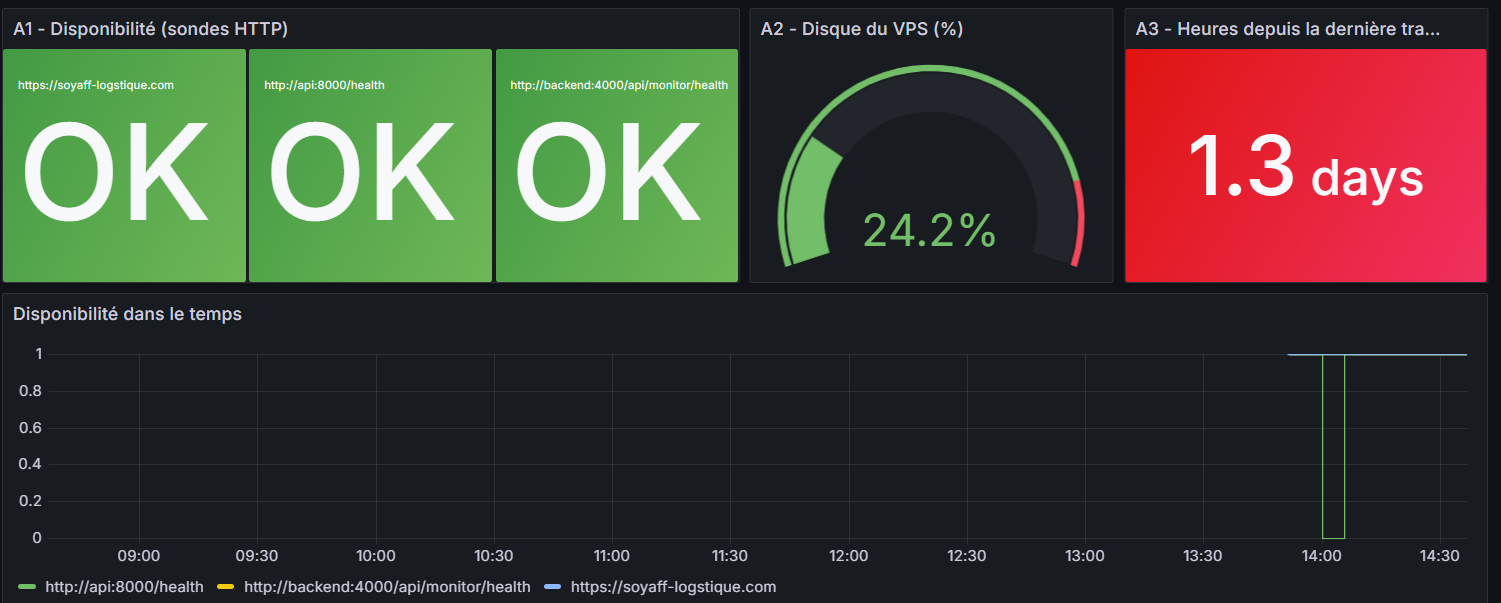
\includegraphics[width=0.85\textwidth]{figures/captures/ops_grafana.png}
    \caption{Tableau de bord Grafana : disponibilité des trois services, disque et fraîcheur des données}
    \label{fig:ops_grafana}
\end{figure}

\begin{figure}[H]
    \centering
    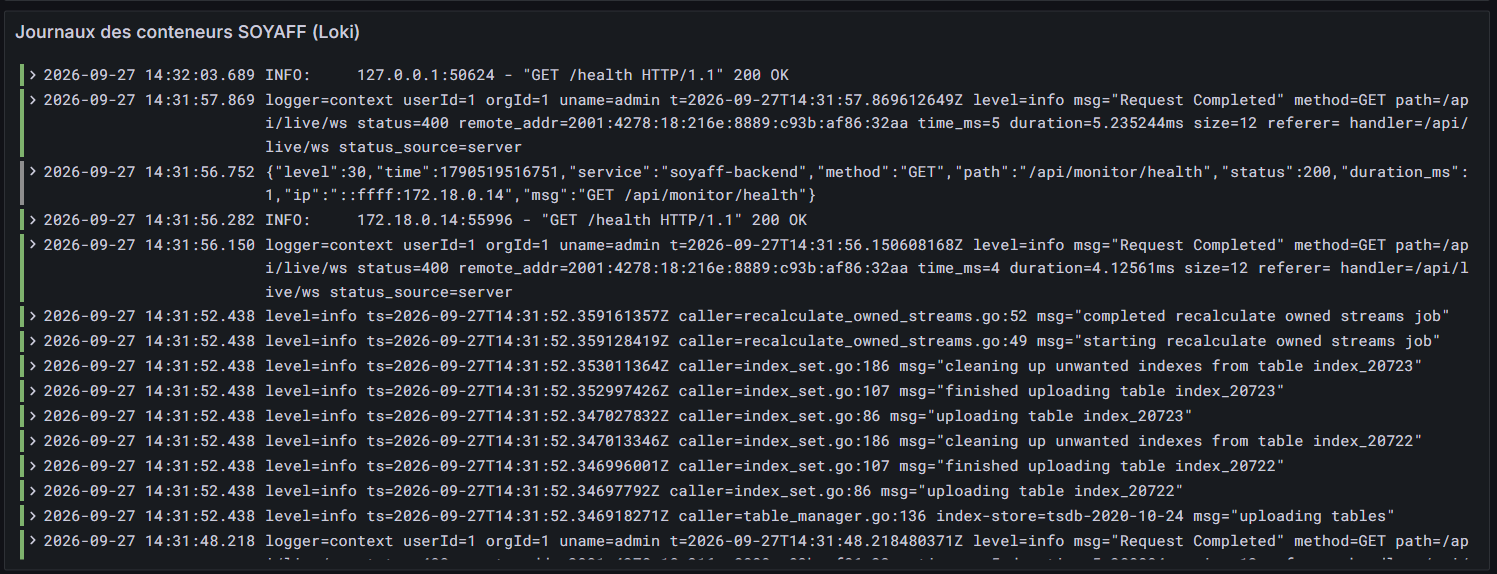
\includegraphics[width=0.85\textwidth]{figures/captures/ops_loki.png}
    \caption{Journaux centralisés des conteneurs dans Loki}
    \label{fig:ops_loki}
\end{figure}

\textbf{Des alertes proactives.} Chaque indicateur porte une règle d'alerte, notifiée sur un canal Telegram par un bot dédié. A1 se déclenche quand un service ne répond plus depuis deux minutes ; A2 quand le disque dépasse 85~\% pendant cinq minutes ; A3 quand aucune transaction n'a été enregistrée depuis plus de 24~heures. Le jeton du bot reste une variable d'environnement, jamais écrite dans le dépôt. Une dégradation n'attend donc plus qu'un utilisateur consulte Grafana pour être connue.

\textbf{Deux pannes provoquées.} Nous avons vérifié ces alertes le 27~septembre~2026 en provoquant deux pannes sur le serveur de production. D'abord, l'arrêt volontaire du service RAG : l'alerte A1 est arrivée sur Telegram à 14:02, puis sa résolution à 14:07 après redémarrage (Figure~\ref{fig:ops_alerte_service}) ; la coupure est visible sur la courbe de disponibilité de la Figure~\ref{fig:ops_grafana}. Ensuite, un fichier temporaire a rempli le disque à 87~\% (Figures~\ref{fig:ops_test_disque_cmd} et~\ref{fig:ops_test_disque_gauge}) : l'alerte A2 est arrivée à 14:33, puis sa résolution après suppression du fichier (Figure~\ref{fig:ops_alerte_disque}).

\begin{figure}[H]
    \centering
    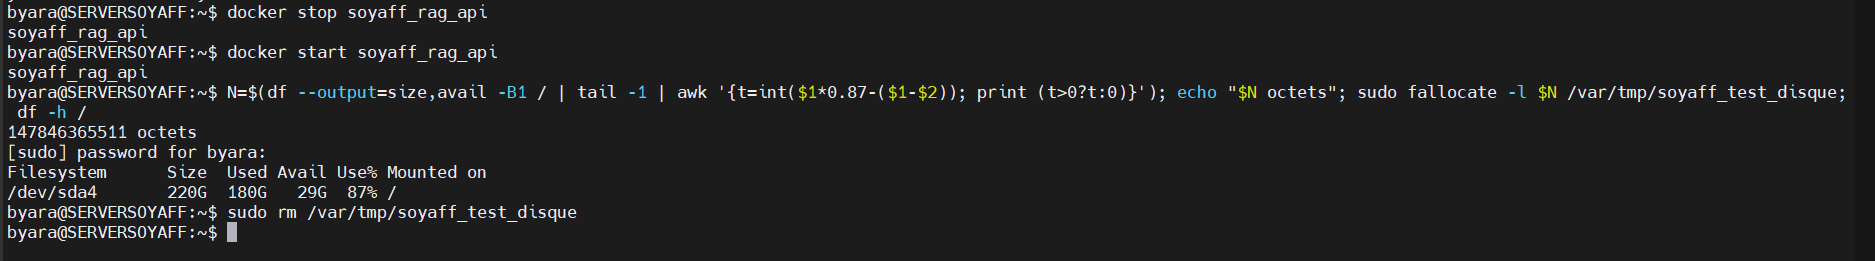
\includegraphics[width=0.9\textwidth]{figures/captures/ops_test_disque_cmd.png}
    \caption{Test de l'alerte disque : arrêt et redémarrage du service RAG, puis remplissage du disque à 87~\%}
    \label{fig:ops_test_disque_cmd}
\end{figure}

\begin{figure}[H]
    \centering
    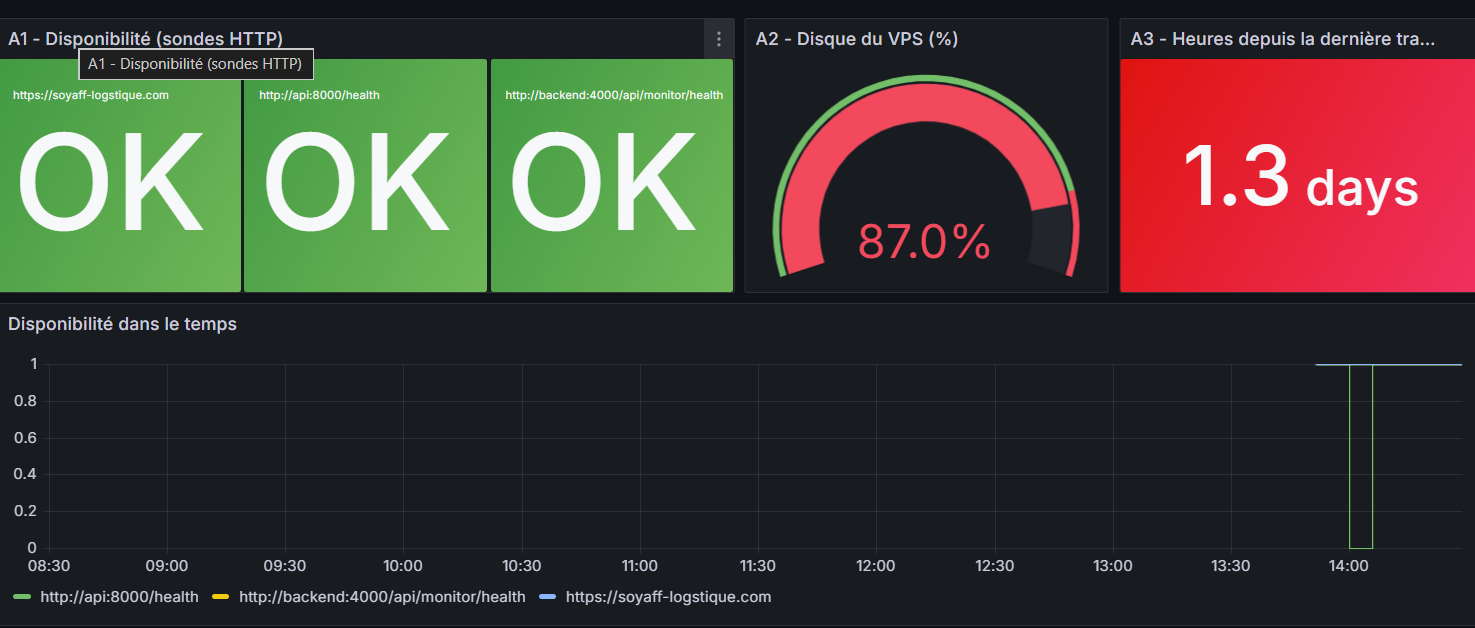
\includegraphics[width=0.7\textwidth]{figures/captures/ops_test_disque_gauge.png}
    \caption{Jauge du disque à 87~\% pendant le test}
    \label{fig:ops_test_disque_gauge}
\end{figure}

\begin{figure}[H]
    \centering
    \begin{minipage}{0.48\textwidth}
        \centering
        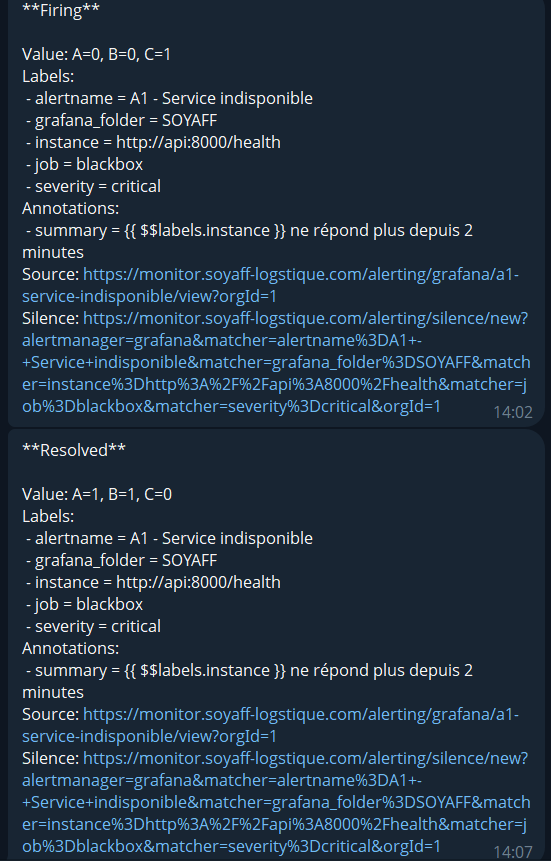
\includegraphics[width=\textwidth]{figures/captures/ops_alerte_service.png}
        \caption{Alerte A1 déclenchée puis résolue (service RAG arrêté)}
        \label{fig:ops_alerte_service}
    \end{minipage}\hfill
    \begin{minipage}{0.48\textwidth}
        \centering
        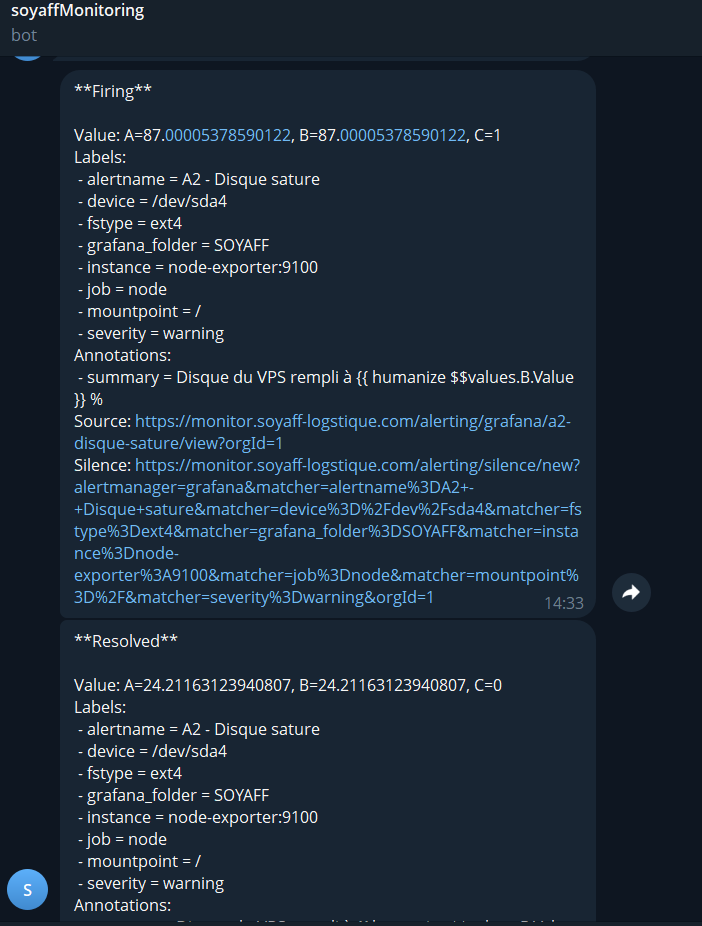
\includegraphics[width=\textwidth]{figures/captures/ops_alerte_disque.png}
        \caption{Alerte A2 déclenchée puis résolue (disque à 87~\%)}
        \label{fig:ops_alerte_disque}
    \end{minipage}
\end{figure}

\textbf{Ce que la supervision couvre.} \texttt{EF-ADM-04} exige de superviser la santé des services ETL, RAG et application web. Les sondes couvrent directement le RAG et l'application ; l'ETL est couvert indirectement par l'alerte de fraîcheur des données, qui ne distingue cependant pas un DAG en échec d'une simple absence de nouveau fichier. \texttt{EF-ADM-04} est donc satisfaite, avec cette réserve pour l'ETL. La même série \texttt{probe\_success} rend la disponibilité (\texttt{ENF-DISP-02}) calculable ; ce calcul relève de la section~\ref{chap:impact_metier}.

\subsection{Sécurité opérationnelle et sauvegarde}
\label{sec:devops_securite}

\textbf{Surface réseau.} Le pare-feu \texttt{UFW} n'ouvre que SSH et les ports~80 et~443 (Figure~\ref{fig:ops_ufw}) ; tous les services sont derrière le Nginx du serveur.

\begin{figure}[H]
    \centering
    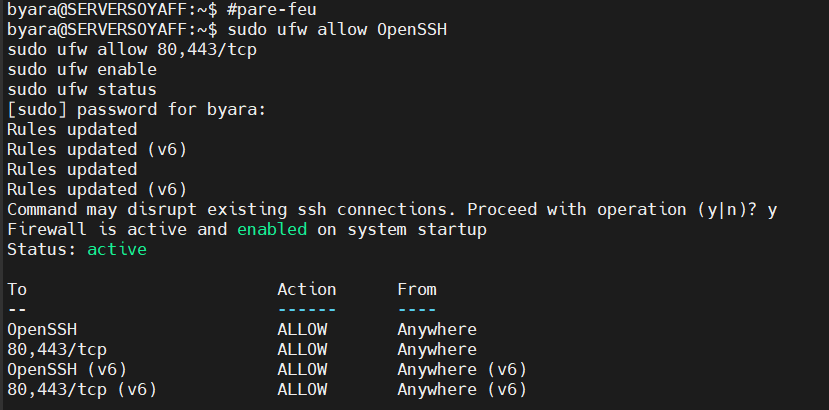
\includegraphics[width=0.55\textwidth]{figures/captures/ops_ufw.png}
    \caption{Pare-feu UFW : seuls SSH, 80 et 443 sont ouverts}
    \label{fig:ops_ufw}
\end{figure}

\textbf{TLS de bout en bout (\texttt{ENF-SEC-05}).} Le trafic des clients passe par Cloudflare. L'ADR-05 avait d'abord retenu le mode \textit{Flexible}, qui laissait en clair le trajet entre Cloudflare et le serveur. Nous sommes passés au mode \textit{Full (strict)} : ce trajet est désormais chiffré lui aussi, et Cloudflare vérifie le certificat du serveur (Figure~\ref{fig:ops_cloudflare}). L'écart à \texttt{ENF-SEC-05} est refermé.

\begin{figure}[H]
    \centering
    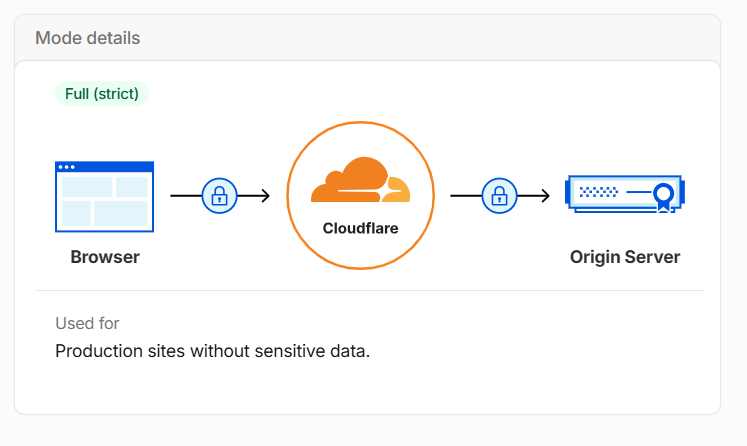
\includegraphics[width=0.45\textwidth]{figures/captures/ops_cloudflare.png}
    \caption{Chiffrement Cloudflare en mode \textit{Full (strict)} : navigateur, Cloudflare et serveur chiffrés de bout en bout}
    \label{fig:ops_cloudflare}
\end{figure}

\textbf{Sauvegarde et restauration (\texttt{EF-ADM-03}, priorité \textit{Must}).} Une tâche planifiée exécute chaque nuit à 02:30 le script \texttt{scripts/backup\_db.sh}. Il produit un \texttt{pg\_dump} de la base, vérifie que l'archive est lisible par \texttt{pg\_restore}, en calcule l'empreinte SHA-256 et conserve quatorze jours d'archives sur le serveur. Il en envoie ensuite une copie hors site, sur l'espace de sauvegarde de 100~Go inclus dans l'offre, par \texttt{rclone} (Figure~\ref{fig:ops_rclone}). Enfin, chaque dimanche à 04:00, une restauration d'essai recharge la dernière archive dans une base jetable, supprimée après vérification. Une sauvegarde jamais restaurée n'est qu'une hypothèse ; celle-ci est éprouvée chaque semaine.

\begin{figure}[H]
    \centering
    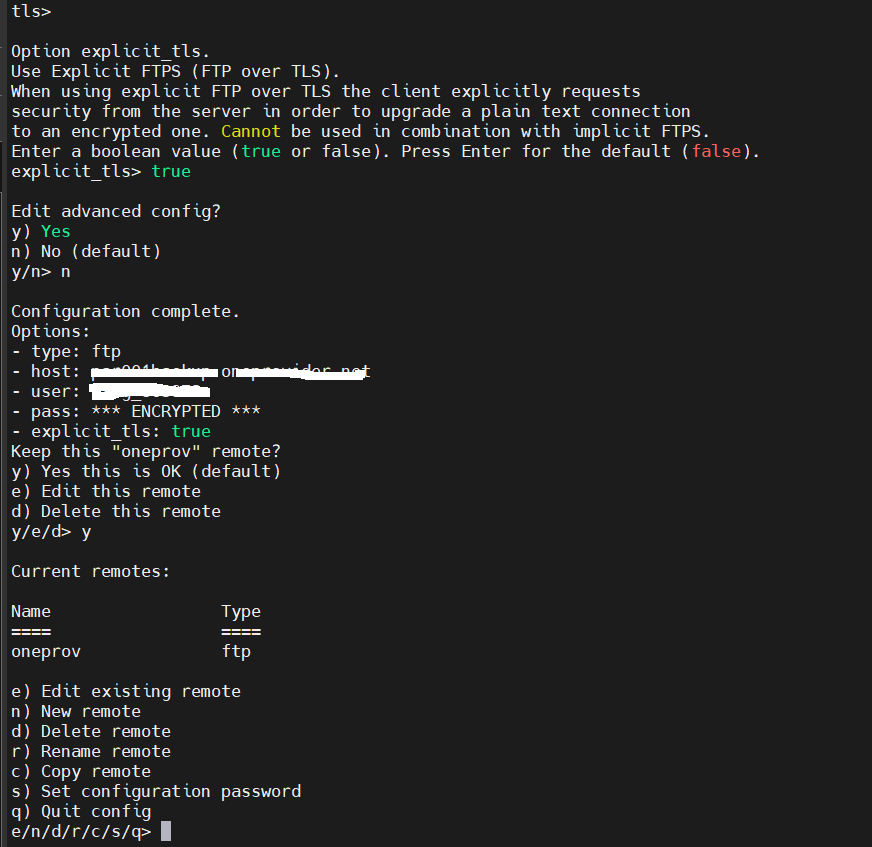
\includegraphics[width=0.45\textwidth]{figures/captures/ops_rclone.png}
    \caption{Configuration de la destination de sauvegarde hors site (\texttt{rclone})}
    \label{fig:ops_rclone}
\end{figure}

\textbf{Piste d'audit.} \texttt{ENF-SEC-04} est satisfaite par la table \texttt{audit\_logs} (section~\ref{chap:webapp}, \S\ref{sec:webapp_rbac}). Les journaux Loki lui sont complémentaires : ils servent l'exploration technique, sans la sémantique métier d'\texttt{audit\_logs}.

\subsection{Écarts, dettes et cohérence}
\label{sec:devops_dettes}

Nous rassemblons ici les écarts du volet DevOps ; leur priorisation est discutée à la section~\ref{chap:discussion}. Ce sont des dettes d'exploitation, pas des défauts de conception : l'infrastructure tient en production, avec des tests bloquants, un déploiement continu, une supervision alertée et une sauvegarde éprouvée.

\begin{itemize}
    \item \textbf{Déploiement sans bascule.} Ni \textit{blue-green}, ni retour arrière automatique ; côté Python, l'échec d'un redémarrage de conteneur ne fait pas échouer le job.
    \item \textbf{Couverture Node non mesurée en CI.} Les tests backend et frontend bloquent le pipeline, mais leur couverture n'est pas calculée, alors que le plancher de 70~\% est déjà déclaré dans \texttt{jest.config.cjs}.
    \item \textbf{\textit{Runner} en mode \texttt{shell}.} Les jobs s'exécutent directement sur le serveur de production, sans isolation par conteneur.
    \item \textbf{Copie hors site non chiffrée.} La base contient des données personnelles (table \texttt{chauffeurs}) ; la copie envoyée sur l'espace FTP de l'hébergeur passe en TLS mais y est stockée en clair. Un chiffrement côté client (\texttt{rclone crypt}) est déjà prévu par le script.
    \item \textbf{Configuration Nginx hors dépôt.} Le Nginx du serveur, qui route les sous-domaines, n'est versionné nulle part.
    \item \textbf{Copie de sauvegarde non chiffrée.} L'archive envoyée hors site contient des données personnelles et n'est pas encore chiffrée.
    \item \textbf{Point de défaillance unique} (ADR-03), inchangé.
\end{itemize}

Plusieurs dettes relevées lors de la première rédaction sont refermées. Le TLS est chiffré de bout en bout (\textit{Full (strict)}). La supervision, autrefois passive, envoie des alertes. La sauvegarde, autrefois absente malgré sa priorité \textit{Must}, est quotidienne, copiée hors site et restaurée chaque semaine. La suite \texttt{pytest}, dont le résultat était masqué, bloque désormais le pipeline avec un plancher de couverture de 95~\%. La pile de supervision est versionnée. S'y ajoutent deux résorptions plus anciennes : la migration de PostgreSQL~13 vers~16 et le passage de l'image \texttt{api} à Python~3.11 sous un utilisateur non-\textit{root}.

\subsection{Synthèse et transition}
\label{sec:devops_synthese_transition}

Nous avons décrit dans cette section la chaîne DevOps qui porte les modules des sections~\ref{chap:etl}, \ref{chap:webapp} et~\ref{chap:ia_rag} : conteneurisation mono-hôte frugale (\S\ref{sec:devops_conteneurisation}), intégration et déploiement continus avec des tests bloquants (\S\ref{sec:devops_cicd}), supervision par sondes, métriques, journaux et alertes (\S\ref{sec:devops_observabilite}), sécurité et sauvegarde (\S\ref{sec:devops_securite}). Les écarts restants (\S\ref{sec:devops_dettes}) bornent ce que l'infrastructure garantit sans remettre en cause la plateforme.

Le chapitre se referme sur une plateforme construite, déployée et exploitée : un pipeline qui consolide les données historiques, une application web qui les expose sous contrôle d'accès, un module conversationnel hybride qui les interroge sans exposer les données sensibles, et l'infrastructure qui porte l'ensemble avec des ressources limitées. Le chapitre~\ref{chap:evaluation} la soumet maintenant à l'épreuve des faits, hypothèse par hypothèse.

